% Autor: Leonhard Segger, Alexander Neuwirth
% Datum: 2017-10-30
\documentclass[
	% Papierformat
	a4paper,
	% Schriftgröße (beliebige Größen mit „fontsize=Xpt“)
	12pt,
	% Schreibt die Papiergröße korrekt ins Ausgabedokument
	pagesize,
	% Sprache für z.B. Babel
	ngerman
]{scrartcl}

% Achtung: Die Reihenfolge der Pakete kann (leider) wichtig sein!
% Insbesondere sollten (so wie hier) babel, fontenc und inputenc (in dieser
% Reihenfolge) als Erstes und hyperref und cleveref (Reihenfolge auch hier
% beachten) als Letztes geladen werden!

\usepackage{tikz}
\usetikzlibrary{calc,patterns,angles,quotes} % loads some tikz extensions\usepackage{tikz}
\usetikzlibrary{babel}

% Silbentrennung etc.; Sprache wird durch Option bei \documentclass festgelegt
\usepackage{babel}
% Verwendung der Zeichentabelle T1 (Sonderzeichen etc.)
\usepackage[T1]{fontenc}
% Legt die Zeichenkodierung der Eingabedatei fest, z.B. UTF-8
\usepackage[utf8]{inputenc}
% Schriftart
\usepackage{lmodern}
% Zusätzliche Sonderzeichen
\usepackage{textcomp}

% Mathepaket (intlimits: Grenzen über/unter Integralzeichen)
\usepackage[intlimits]{amsmath}
% Ermöglicht die Nutzung von \SI{Zahl}{Einheit} u.a.
\usepackage{siunitx}
% Zum flexiblen Einbinden von Grafiken (\includegraphics)
\usepackage{graphicx}
% Abbildungen im Fließtext
\usepackage{wrapfig}
% Abbildungen nebeneinander (subfigure, subtable)
\usepackage{subcaption}
% Funktionen für Anführungszeichen
\usepackage{csquotes}
\MakeOuterQuote{"}
% Zitieren, Bibliografie
\usepackage[sorting=none]{biblatex}

\usepackage{multirow}% http://ctan.org/pkg/multirow


% Zur Darstellung von Webadressen
\usepackage{url}
%chemische Formeln
\usepackage[version=4]{mhchem}
% siunitx: Deutsche Ausgabe, Messfehler getrennt mit ± ausgeben
\usepackage{floatrow}
\floatsetup[table]{capposition=top}
\usepackage{float}
% Verlinkt Textstellen im PDF-Dokument
\usepackage[unicode]{hyperref}
% "Schlaue" Referenzen (nach hyperref laden!)
\usepackage{cleveref}
\sisetup{
	locale=DE,
	separate-uncertainty
}
\bibliography{BA-C-04_MP6_07-01-2019_References}

\begin{document}

	\begin{titlepage}
		\centering
		{\scshape\LARGE Versuchsbericht zu \par}
		\vspace{1cm}
		{\scshape\huge MP6 - Metallische Gläser \par}
		\vspace{2.5cm}
		{\LARGE Gruppe BA-C-04 \par}
		\vspace{0.5cm}

		{\large Alexander Neuwirth (E-Mail: a\_neuw01@wwu.de) \par}
		{\large Leonhard Segger (E-Mail: l\_segg03@uni-muenster.de) \par}
		\vfill

		durchgeführt am 07.01.2019\par
		betreut von\par
		{\large Manoel da Silva Pinto}

		\vfill

		{\large \today\par}
	\end{titlepage}
	\tableofcontents
	\newpage

	\section{Kurzfassung}
	% Hypothese	und deren Ergebnis, wenn Hypothese ist, dass nur Theorie erfüllt, sagen: Erwartung: Theorie aus einführung (mit reflink) erfüllt
	% Ergebnisse, auch Zahlen, mindestens wenn's halbwegs Sinn ergibt
	% Was wurde gemacht
	% manche leute wollen Passiv oder "man", manche nicht
	Metallische Gläser zeigen einige Eigenschaften, die sie von anderen Festkörpern unterscheiden.
	In diesem Versuchsbericht wird vor allem der Vergleich zu kristallinen Festkörpern vollzogen.
	Zunächst wird dazu mit einem Leistungskalorimeter der Wärmefluss beim Erhitzen einer kristallinen und einer amorphen, gläsernen Probe aufgezeichnet und daraus im Falle der kristallinen Probe Schmelz- und Erstarrungsenthalpie berechnet und im Fall der amorphen Probe die Kristallisationsenthalpie bestimmt.
	Hier kann gezeigt werden, dass der Übergang vom Kristall in die Schmelze reversibel und der Übergang vom Glas zum Kristall irreversibel ist.
	Dass die Kristallisationstemperatur der amorphen Probe mit der Heizrate steigt, wird nicht hinreichend signifikant gezeigt.
	Außerdem wird die Aktivierungsenthalpie nach Kissinger bestimmt.

	Im nächsten Versuchsteil wird eine amorphe PdNiP-Probe und eine kristalline PdNiP-Probe unter monochromatischer Röntgenstrahlung in Abhängigkeit vom Einstrahlwinkel untersucht.
	Dabei kann gezeigt werden, dass durch diese Untersuchung gut zwischen kristalliner und gläserner Phase unterschieden werden kann.
	%Ein Vergleich der Gitterkonstanten bzw. mittleren Atomabstände

	Zuletzt wird amorphes PdNiP und kristallines Nickel mit einem Mikroindenter untersucht und bestätigt, dass die amorphe Struktur eine größere Vickershärte zufolge hat.

  \section{Theorie}
	%TODO noch sagen, dass halt nur bei Metallen
	% wdh. Texte
	% wdh. Besprechung

	\subsection{Phasenübergang}

	Für das Verständnis des Verhaltens von metallischen Gläsern ist die Keimbildungstheorie fundamental.
	Dieser geht die Annahme voraus, dass der Kristallisationsprozess von kleinsten Keimen (Verunreinigungen) ausgeht und sich dann durch die gesamte Probe fortsetzt.
	Um diesen Vorgang zu beschreiben, wird die Gibbs-Energie (auch freie Enthalpie) verwendet, welche in einem geschlossenen System konstanter Temperatur und konstanten Drucks minimiert wird.
	Diese Minimierung lässt sich als treibende Kraft des Kristallisationsprozesses verstehen.


	Die Änderung der Gibbs-Energie ergibt
	\begin{equation}
		\label{eq_gibbs}
		\Delta G = - \frac{4 \pi}{3} r^3 \Delta G_\text{v} + 4 \pi r^2 \sigma ,
	\end{equation}
	wobei $r$ der Radius des sphärisch angenommenen Keims ist und $\Delta G_\text{v} = g_\text{s} - g_\text{k}$ (freie Enthalpie der Schmelze und des Kristalls) als Änderung der spezifischen freien Enthalpie die treibende Kraft der Umwandlung pro Volumeneinheit darstellt.

	\begin{figure}[H]
			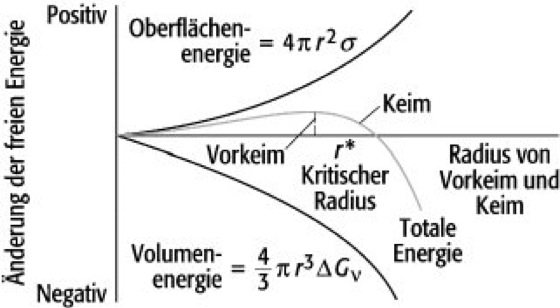
\includegraphics[width= 0.5 \linewidth]{img/radius}
			\caption{
			Darstellung der Änderung der freien Enthalpie in Abhängigkeit von der Keimgröße.
			Es ist leicht zu erkennen, dass ein kritischer Radius überschritten werden muss, damit der Keim stabil ist und wachsen kann.
			\cite{radius_enthalpie}
			}
			\label{fig_radius_enthalpie}
	\end{figure}

	Daraus ergibt sich, wie in \cref{fig_radius_enthalpie} zu erkennen ist, ein kritischer Radius, unter dem Keime nicht stabil sind und keine Kristallisation stattfinden kann.
	Dies ist darin begründet, dass die Grenzfläche zwischen kristalliner und amorpher Phase energetisch ungünstiger als beide Phasen ist.
	Da das Volumen mit $r^3$ und die Oberfläche mit $r^2$ geht, ist eine Erhöhung des Keimradius also erst ab einem bestimmten Radius energetisch günstig.

	Aus diesen Erkenntnissen folgt, dass für die Frage, ob eine Abkühlende Schmelze kristallisiert, die Geschwindigkeit des Entstehens und Größe der Keime sowie die Abkühlrate relevant sind.
	Wenn die Schmelze schnell genug abgekühlt wird bzw. die Probe ausreichend rein ist, können sich keine ausreichend große Keime bilden und sie erstarrt in amorpher Form (vgl. \cref{fig_kristallisierung}).

	\begin{figure}[H]
			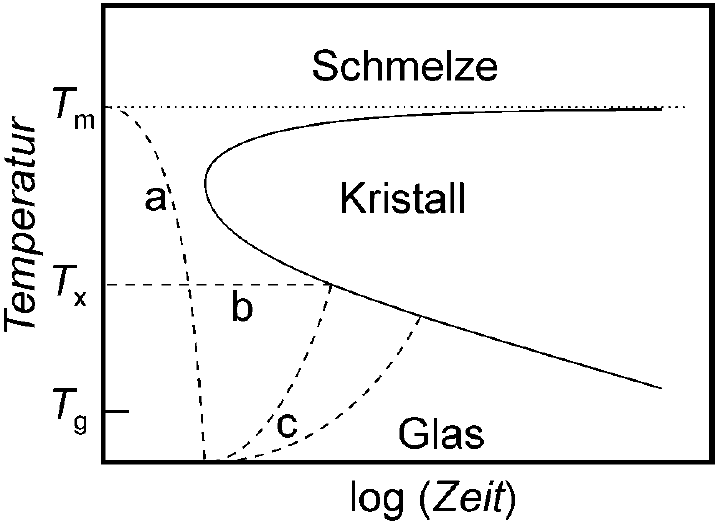
\includegraphics[width= 0.7 \linewidth]{img/kristallisierung}
			\caption{
			ZTU-Diagramm zu Kristallisation und Glasbildung
			a) schnelles Abschrecken
			b) isotherme Kristallisation
			c) Kristallisation für schnelle (links) und langsame (rechts) Aufheizrate
			\cite{anleitung}
			}
			\label{fig_kristallisierung}
	\end{figure}

	In \cref{fig_kristallisierung} ist als c) auch der umgekehrte Prozess dargestellt, welcher in diesem Versuch untersucht wird.
	Das Erhitzen eines Metalls in Glasphase führt dazu, dass es in den Bereich der unterkühlten Schmelze gerät, in der der oben beschriebene Keimbildungsprozess zur Kristallisation führen kann.
	Je schneller das Erhitzen stattfindet, desto eher kristallisiert das Glas, aber auch ein geringes Erhitzen gefolgt von einem Konstanthalten der Temperatur führt nach ausreichender Zeit zu Kristallisation.
	Demnach ist auch die bei der Kristallisation vorliegende Temperatur abhängig von der Heizrate.
	Dieser Prozess ist irreversibel, weshalb ein Senken der Temperatur nicht wieder in die Glasphase führt.
	Hierfür wäre ein Schmelzen gefolgt vom oben geschilderte Prozess der schnellen Abkühlung erforderlich.

	Die Schmelzenthalpie eines Metalls, das nicht in die Glasphase gerät, ist dem hingegen nur materialabhängig und kann mit Literaturwerten verglichen werden, da der Übergang von Schmelze zu Kristall reversibel ist.
	Hier ist also zu erwarten, dass die Schmelzenthalpie der Kristallisationsenthalpie entspricht.

	\subsection{Röntgendiffraktometrie}
	Da ein amorpher Festkörper lediglich eine Nahordnung der Atome besitzen kann, während ein Kristall eine regelmäßige Gitterstruktur aufweist, ist zu erwarten, dass sich der amorphe Festkörper unter monochromatischem Röntgenlicht eher wie ein pulverisierter Kristall verhält und sich ein kontinuierliches Spektrum zeigt.
	Beim Kristall hingegen sind nur einige scharfe Reflexe zu erwarten, bei denen die Bragg-Gleichung erfüllt ist.
	Aus der Position des Maximums beim amorphen Kristall lässt sich gemäß der Bragg-Gleichung der Mittlere Atomabstand berechnen.


	%\subsection{Vickershärte}

	\section{Methoden} %TODO Ziele angeben
	% Bilder von der Website klauen
	% einer will Präsens
	Es sollen drei verschiedene Untersuchungen bezüglich des Verhaltens von metallischen Gläsern durchgeführt werden.
	Hierzu wird als Vertreter der metallischen Gläser PdNiP verwendet.

	\subsection{Kalorimetrie}
	Es wird ein Leistungskalorimeter eingesetzt, um den Wärmefluss beim Erhitzen von verschiedenen Stoffen zu untersuchen.
	Zunächst wird eine Bleiprobe, die sich bereits in einem Tiegel befindet, im Vergleich zu einem Referenztiegel untersucht.
	Bei dieser wird keine gläserne Phase erwartet, da dies ein Erhitzen über den Schmelzpunkt gefolgt von einem schnelleren Abkühlen, als es mit diesem oder einem anderen bekannten Aufbau möglich ist, erfordern würde.
	Es wird ein Messzyklus durchgeführt und das auf der Probe angegebene Gewicht notiert.

	Dann werden von einem Band aus amorphem PdNiP drei ungefähr gleich große Stücke mit einer Zange abgekniffen, gewogen und in Tiegeln verschlossen.
	Diese werden im Vergleich zu einem leeren Referenztiegel im Kalorimeter bei je unterschiedlicher Heizrate untersucht.
 	Hier werden zwei Messzyklen aufgenommen.

	\subsection{Röntgendiffraktometrie} %lul steht in der Anleitung mindestens einmal falsch geschrieben
	In einem Röntgendiffraktometer (Kupfer-Anode, $\text{K}_\alpha$-Linie) wird im Debye-Scherrer-Verfahren die Röntgenbeugung in Abhängigkeit vom Einstrahlwinkel unter monochromatischer Röntgenstrahlung gemessen.
	Dabei wird eine amorphe und eine kristalline PdNiP-Probe untersucht.
	Beide sind nicht pulverisiert.	% weil pulver erwartung, dass bei kristall nichts exaktes

	\subsection{Messung der Vickershärte}
 	Es wird ein Mikroindenter verwendet, um die Vickershärte einer Probe aus kristallinem Nickel und einer aus amorphem PdNiP zu bestimmen. % das steht in der Anleitung, aber an den Daten steht was von Paradin-Phosphor (was nicht existiert) und Ni.
	Dazu wird ein Diamant in Form einer vierseitigen Pyramide mit einem Öffnungswinkel von \SI{136}{\degree} für \SI{5}{s} mit einer Kraft von \SI{0.5}{kgf} auf die Probe gedrückt.
	Dann wird mit einem Mikroskop die Länge der beiden Diagonalen gemessen.
	Das verwendete Gerät errechnet dann aus diesen Werten die Vickershärte.
	Es werden jeweils \num{10} Messungen durchgeführt, um einen Mittelwert bilden zu können.

	\section{Ergebnisse und Diskussion}

	\subsection{Kalorimetrie}
	\subsubsection{Unsicherheiten}
	Folgende Unsicherheiten werden angenommen:
	\begin{description}
		\item[Waage:]  Digitalanzeige, Rechteckverteilung, $u(m)=\SI{3}{\mu g}$
		\item[Thermometer:] digital, Rechteckverteilung, $u(T)=\SI{0.003}{K}$
		\item[Leistungsdifferenzkalorimeter:] digital, Rechteckverteilung, $u(\Phi)=\SI{0.03}{\mu W}$
	\end{description}
	\subsubsection{Beobachtung und Datenanalyse}
	\subsubsection*{Vergleichsprobe} \label{ssss_vergleich}
	In \cref{fig_thermo_blei} ist der temperaturabhängige Verlauf des Wärmeflusses beim Aufheizen und Abkühlen  der Bleiprobe abgebildet.
	Um die Schmelztemperatur zu bestimmen wurden an die Aufheizkurve zwei Geraden (Basislinie und Peak) angepasst (grün).
	Der Schnittpunkt der linearen Funktionen liefert die Schmelztemperatur $T_s= \SI{327.2+-3.1}{\celsius}$.
	Analog erhält man die Erstarrungstemperatur $T_e = \SI{314.1+-2.8}{\celsius}$.


	\begin{figure}[H]
			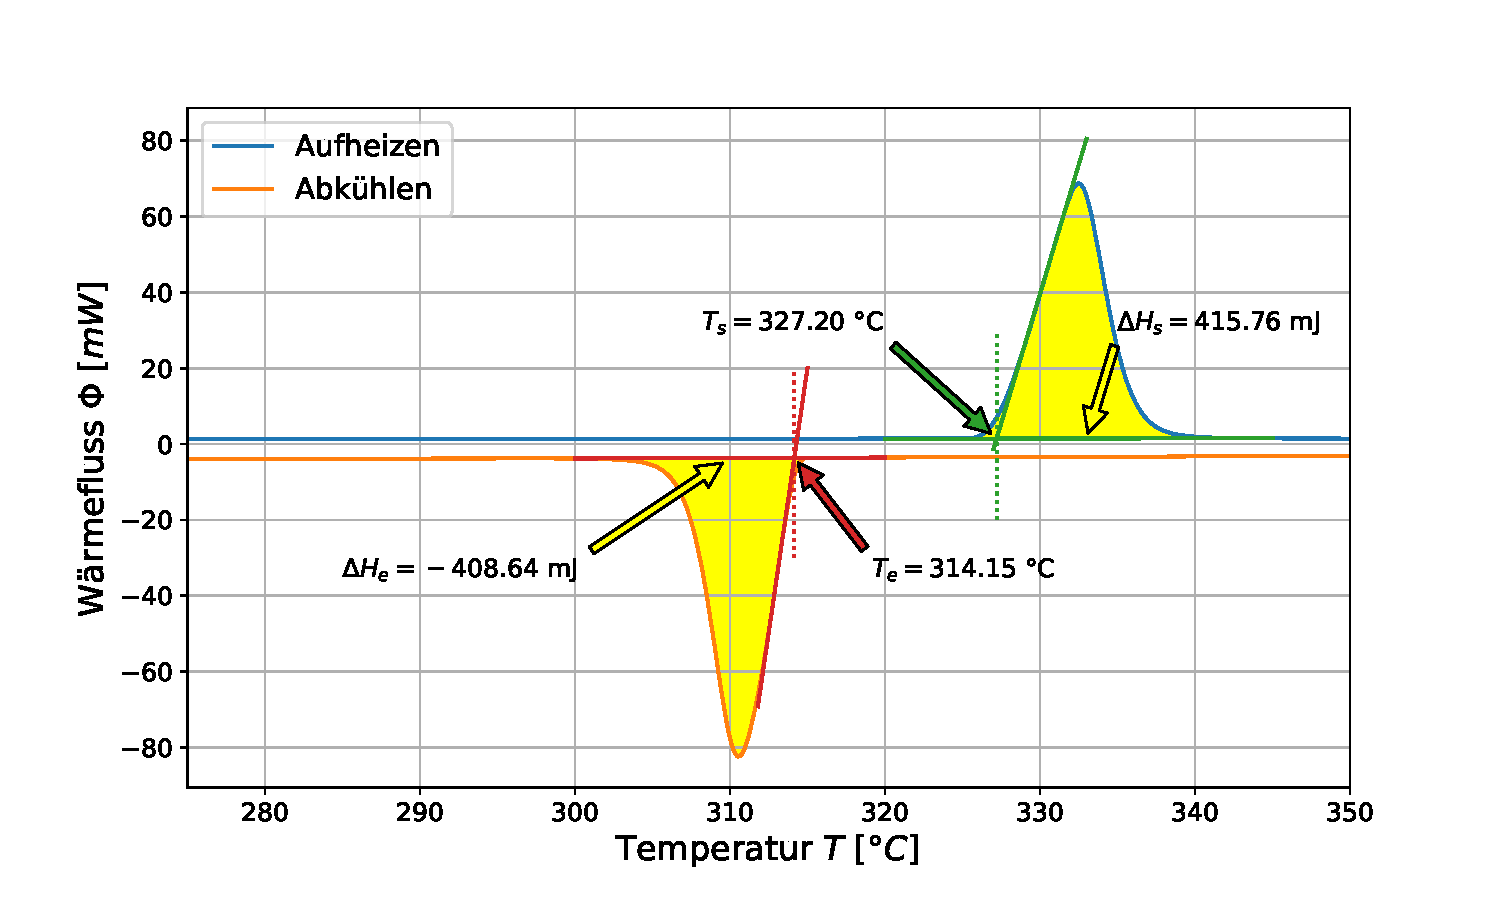
\includegraphics[width=\linewidth]{img/Kalorimetrie_blei.pdf}
			\caption{
			Thermogramm der Bleiprobe bei einer Heiz- bzw. Abkühlrate $\alpha =\SI{50}{K/min}$.
			Der rote (grüne) Pfeil zeigt auf den Schnittpunkt der linearisieren Peaksteigung und Basislinie.
			Er gibt also die Erstarrungstemperatur (Schmelztemperatur) an.
			Die gelben Pfeile beschreien die mittels \cref{eq_enth} berechneten Enthalpien im jeweiligen farblich gekennzeichneten Bereich zwischen Basislinie und Peak.
			Die Unsicherheiten sind kleiner als die Symbolgröße.
			}
			\label{fig_thermo_blei}
	\end{figure}

	Die Schmelzenthalpie ist gegeben durch die eingeschlossen Fläche zwischen Basislinie und Peak, die hier durch eine Summe genähert wird, was aufgrund des geringen Abstands der Messwerte in T eine gute Näherung ist:
	\begin{equation}
			\label{eq_enth}
			\Delta H = \frac{1}{\alpha} \int \Phi(T) dT \approx \frac{1}{\alpha} \sum_{i=1}^{N-1} \Phi(T_i) (T_i-T_{i+1})
	\end{equation}
	Dabei ist $\alpha=\SI{50}{K/min}$ die Rate der Temperaturänderung.
	Die Masse des Bleis ist mit \SI{16.62}{mg} angegeben, woraus sich die spezifische und daraus mit der Molmasse \SI{207.2}{g/mol} die molare Enthalpie bestimmen lässt. % source 4 molmasse https://www.lenntech.de/pse/elemente/pb.htm
	Diese sind in \cref{tb_enthal_blei} aufgeführt.
\begin{table}[H]
		\centering
		\begin{tabular}{c | c | c | c  }
			 &$\Delta H$ in \si{mJ}& $\Delta h$ in \si{J/g} &$\Delta H_m$ in \si{kJ/mol}\\ \hline
			 Schmelzenthalpie& \SI{415.8+-2.8}{}&\SI{25.01+-0.17}{}& \SI{5.182+-0.035}{} \\
			 Erstarrungsenthalpie&\SI{-408.6+-0.7}{}&\SI{-24.58+-0.04}{}&\SI{-5.093+-0.008}{} \\
		\end{tabular}
		\caption{
		Verschiedene gemessene Enthalpien der Bleiprobe unnormiert, normiert auf ein Gramm und auf ein Mol.
		}
		\label{tb_enthal_blei}
\end{table}
 % signi weg in den Tabellen??? >> halte ich für egal, sag halt sonst in caption: Ist orientierte Fläche, deshalb negativ.
	\subsubsection*{PdNiP-Probe}
	Es wurde der Wärmefluss in Abhängigkeit von der Temperatur für verschieden schwere PdNiP-Proben gemessen.
	Jede Probe wurde zweimal erhitzt und wieder abgekühlt.
	In \crefrange{fig_themo_pdnip_20}{fig_themo_pdnip_100} ist die Differenz des zweiten Aufheizen von dem ersten abgebildet.
	Die Kristallisationspeaktemperaturen sind in blau gekennzeichnet.
	Die Kristallisationsenthalpie ist in gelb markiert und berechnet sich analog zur \nameref{ssss_vergleich}.
	Der orange Pfeil zeigt auf die Kristallisationstemperatur, die sich ebenfalls analog ergibt.
	Die Glasübergangstemperatur befindet sich an der Stelle an welcher der Wärmefluss mittig zwischen der roten und der grünen Gerade.

	\begin{figure}[H]
			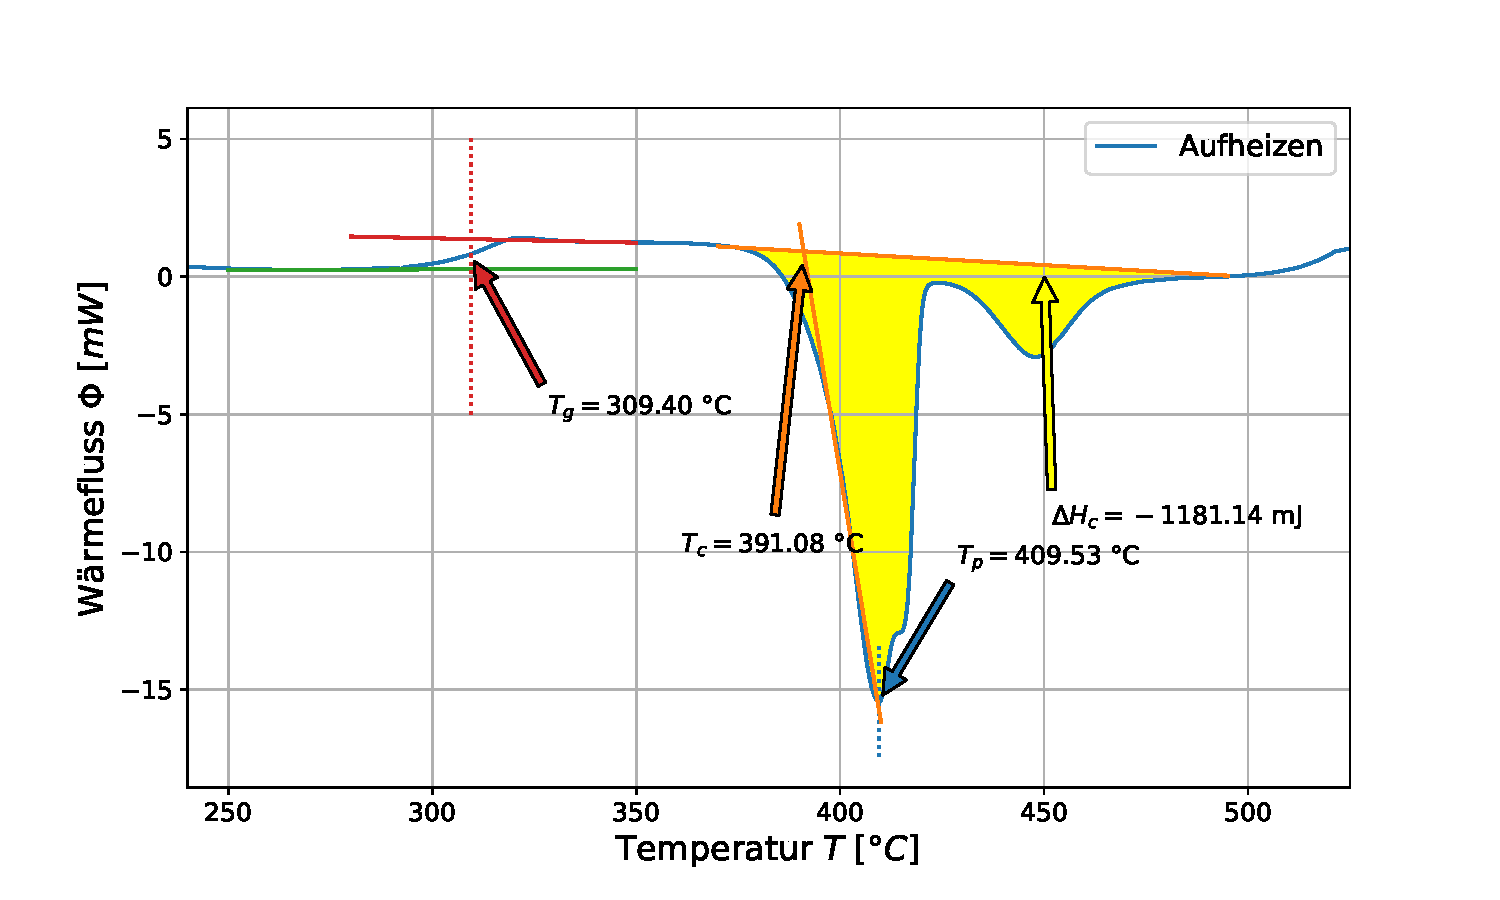
\includegraphics[width=\linewidth]{img/Kalorimetrie_pdnip_20.pdf}
			\caption{
				Thermogramm der \SI{10.99}{mg} PdNiP-Probe bei einer Heizrate $\alpha = \SI{20}{K/min}$.
			Die Unsicherheiten sind kleiner als die Symbolgröße.
			}
			\label{fig_themo_pdnip_20}
		\end{figure}
	\begin{figure}[H]
			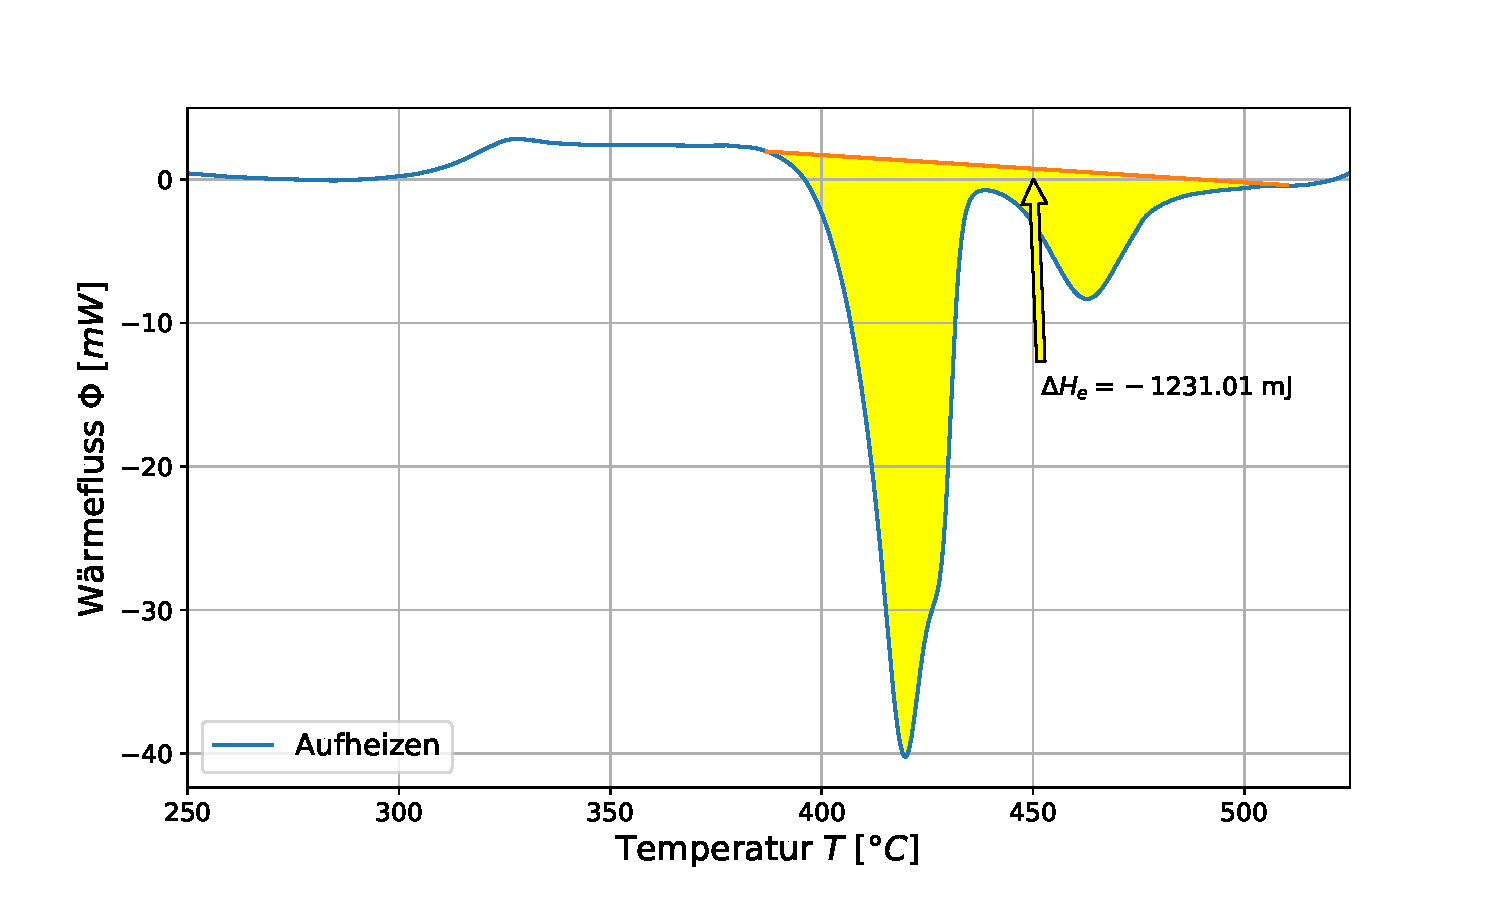
\includegraphics[width=\linewidth]{img/Kalorimetrie_pdnip_50.pdf}
			\caption{
				Thermogramm der \SI{11.52}{mg} PdNiP-Probe bei einer Heizrate $\alpha = \SI{50}{K/min}$.
			Die Unsicherheiten sind kleiner als die Symbolgröße.
			}
			\label{fig_themo_pdnip_50}
		\end{figure}
	\begin{figure}[H]
			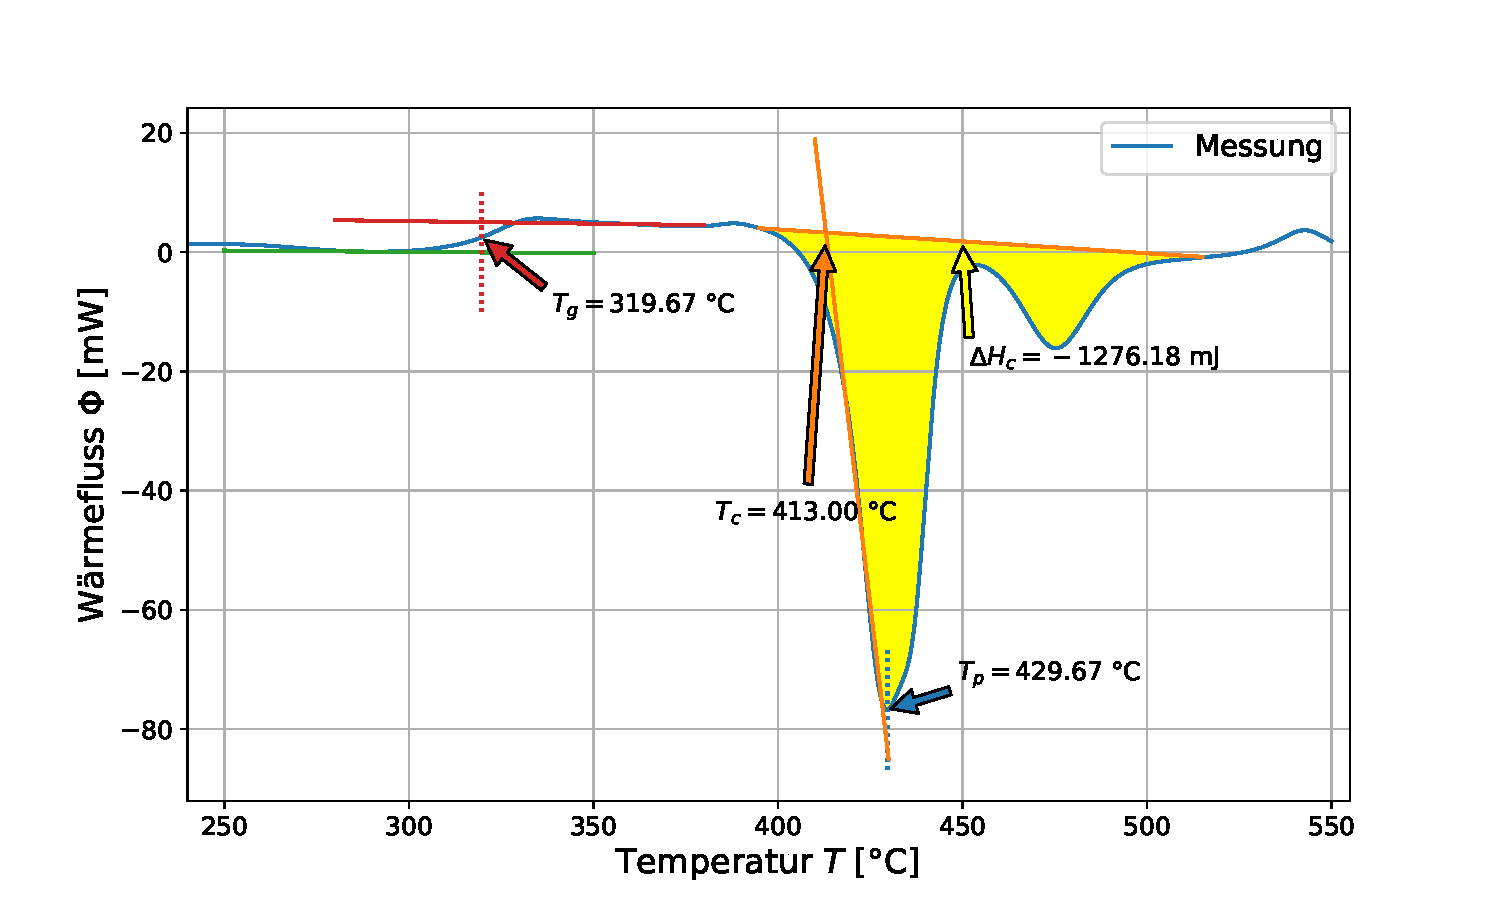
\includegraphics[width=\linewidth]{img/Kalorimetrie_pdnip_100.pdf}
			\caption{
				Thermogramm der \SI{11.94}{mg} PdNiP-Probe bei einer Heizrate $\alpha = \SI{100}{K/min}$.
			Die Unsicherheiten sind kleiner als die Symbolgröße.
			}
			\label{fig_themo_pdnip_100}
	\end{figure}
	Die spezifische und molare Kristallisationsenthalpie lässt sich erneut mit Masse und molarer Masse der Probe bestimmen.
	Die molare Masse $M$ ergibt sich als Summe der molaren Massen der Bestandteile.
	Sie beträgt somit $M=\SI{196.1}{g/mol}$. % src: https://www.lenntech.de/pse/elemente/p.htm
\begin{table}[H]
		\centering
		\begin{tabular}{c | c | c | c  }
			 Masse $m$ &$\Delta H$& $\Delta h$  &$\Delta H_m$ \\ \hline
			 \SI{10.99}{mg}& \SI{-1181+-14}{mJ}&\SI{-107.5+-1.3}{J/g}& \SI{-21.1+-0.3}{kJ/mol} \\
			 \SI{11.52}{mg}& \SI{-1231+-13}{mJ}&\SI{-106.9+-1.1}{J/g}& \SI{-21.0+-0.2}{kJ/mol} \\
			 \SI{11.94}{mg}& \SI{-1276+-50}{mJ}&\SI{-106.9+-4.2}{J/g}& \SI{-21.0+-0.8}{kJ/mol} \\
		\end{tabular}
		\caption{
		Verschiedene gemessene Kristallisationsenthalpien der PdNiP-Proben.
		}
		\label{tb_enthal_pdnip}
\end{table}

	Um die Aktivierungsenthalpie $Q$ nach Kissinger zu erhalten, wird gemäß \cref{eq_linear} in \cref{fig_thermo_kissinger} linearisiert.
	\begin{equation}
		\label{eq_linear}
			\ln{\frac{\alpha}{T_p^2}} = -\frac{Q}{RT_p} + C
	\end{equation}
	Hier bei ist $T_p$ die Kristallisationspeaktemperatur in Kelvin und $\alpha$ die zur selben Messung gehörende Heizrate in \si{K/min}.
	$R=\SI{8.31446}{J/molK}$ ist die allgemeine Gaskonstante und C eine beliebige Konstante.
	Das Resultat ist eine Aktivierungsenthalpie $Q=\SI{289+-18}{kJ/mol}$.

		\begin{figure}[H]
			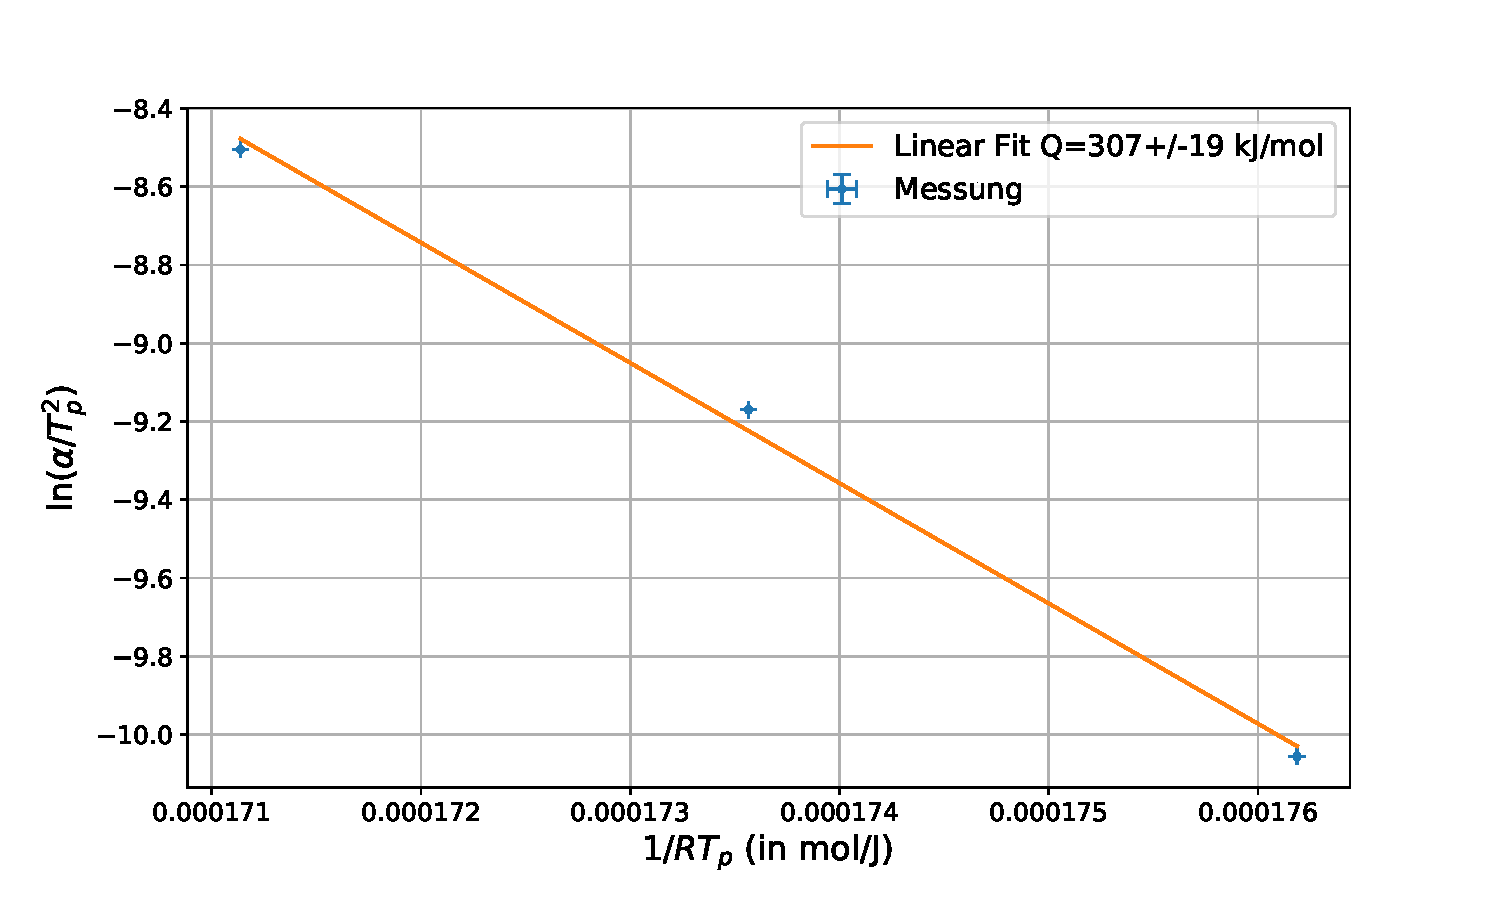
\includegraphics[width=\linewidth]{img/Kalorimetrie_kissinger.pdf}
			\caption{
			Linearisierung der Kristallisationspeaktemperaturen und Heizraten nach \cref{eq_linear} zur Bestimmung der Aktivierungsenthalpie nach Kissinger.
			}
			\label{fig_thermo_kissinger}
		\end{figure}


	\subsubsection{Diskussion}

	% erwartung dass Q größer H ist, nach Anleitungs Bild >> nee
	%TODO Übersteuerung am Ende durch Umschalten von Heizen zu Kühlen.
	\subsubsection*{Vergleichsprobe}
	Es war zu erwarten, dass bei der Untersuchung von Blei die Schmelzenthalpie der Erstarrungsenthalpie entspricht, da es sich um einen reversiblen Vorgang handelt.
	Die Vorzeichen kommen dadurch zustande, dass beim Schmelzen eine zusätzliche Wärme zugeführt werden muss (endotherm), da die Schmelze energetisch ungünstiger als das Kristallgitter ist und dementsprechend beim Erstarren Wärme frei wird (exotherm).
	Wenn man die Messwerte dafür in \cref{tb_enthal_blei} betrachtet, stellt man fest, dass dies innerhalb der doppelten Unsicherheit nicht der Fall ist.
	Wenn man jedoch die dreifache Unsicherheit verwendet, überschneiden sich die Unsicherheitsintervall, weshalb hier kein Widerspruch festgestellt werden kann.
	Der Literaturwert der auf ein Mol normierten Schmelzenthalpie von Blei beträgt \SI{5.12}{\kilo \joule \per \mol} \cite{blei_enthalpie}.
	Wenn man hierfür einen Rundungsunsicherheit annimmt, deckt sich dies mit dem Messwert von \SI{5,182 \pm 0,035}{\kilo \joule \per \mol}. % könnte der dude natrülich sagen wir sollen genauere Literatur verwenden, aber ist mir jedenfalls Wurst ...
	% sollen wir standardmässig / oder \per in SI verwenden, weil 1 ist / anderes ^-1 , aber nicht so wichtig >> ja

	\subsubsection*{PdNiP-Probe}
	Wenn man \crefrange{fig_themo_pdnip_20}{fig_themo_pdnip_100} anschaut, ist zu beobachten, dass bei der Kristallisation (exotherm) nicht wie zu erwarten war ein negativer Peak, sondern zwei eindeutiger und ein dritter an der Flanke des größeren zu vermutender gemessen wurden. %TODO so fine?
	Die ist vermutlich darauf zurückzuführen, dass im Glas Bereiche vorhanden sind, die vornehmlich aus Nickel- und Phosphoratomen bestehen, sowie Bereiche, die vornehmlich aus Nickel- und Palladiumatomen bestehen, was zu zwei verschiedenen Kristallisationsenthalpien für die beiden Bereiche führen würde.
	Der fragliche dritte Peak lässt dann vermuten, dass auch einige wenige Bereiche, die vornehmlich aus Phosphor und Palladium oder allen drei Elementen bestehen, existieren. %TODO so fine?

	Da die Proben alle aus dem selben Material bestehen, und die Kristallisationsenthalpie die Energie darstellt, die frei wird, weil das Metall in einen günstigeren Zustand übergeht, wurde erwartet, dass die normierten Kristallisationsenthalpien in \cref{tb_enthal_pdnip} bei allen drei Proben im Rahmen der Unsicherheiten gleich sind.
	Dies ist der Fall.

	Für die Kristallisationstemperatur war aufgrund von \cref{fig_kristallisierung} zu erwarten, dass sie bei einer höheren Heizrate höher ist.
	Dazu sind die gemessenen Kristallisationstemperaturen in \cref{tb_kristall_temp} eingetragen.
	Der Anstieg der Kristallisationstemperatur mit der Heizrate lässt sich zwar feststellen, ist aber aufgrund der großen Unsicherheiten nicht signifikant.
	Die großen Unsicherheiten kommen durch die linear interpolierte Basislinie (Tangentenkonstruktion) zustande.

	\begin{table}[H]
			\centering
			\begin{tabular}{c | c | c | c  }
				 Heizrate & \SI{20}{\kelvin \per \minute} & \SI{50}{\kelvin \per \minute}  & \SI{100}{\kelvin \per \minute} \\ \hline
				 $T_c$ & \SI{391 \pm 6}{\celsius}&\SI{403 \pm 8}{\celsius} & \SI{-413 \pm 18}{\celsius}
			\end{tabular}
			\caption{
			Kristallisationstemperaturen bei den drei untersuchten Heizraten. Die Unsicherheiten ergeben sich aus dem Fit.
			}
			\label{tb_kristall_temp}
	\end{table}

	Dass beim Abkühlen der Probe das PdNiP keinen positiven Wärmefluss im Vergleich zum Referenztiegel aufweist, entspricht den Erwartungen, da der Übergang von Glas zu Kristall irreversibel ist.

	Der Vergleich der Kristallisationsenthalpie der amorphen Probe (vgl. \cref{tb_enthal_pdnip}) mit der Aktivierungsenthalpie nach Kissinger (\SI{289 \pm 18}{\kilo \joule \per \mol}) führt dazu, dass die Aktivierungsenthalpie etwa \SI{13,8}{}-mal so groß wie die Kristallisationsenthalpie ist.
	Es war kein expliziter Zusammenhang zwischen Kristallisationsenthalpie und Aktivierungsenthalpie zu erwarten.
	Beide Energien addiert ergeben die Energie, die aufgebracht werden kann, um den Potenzialberg zu überwinden und die Kristallisationsenthalpie ist die Energie, die in der Differenz zu der, die nach dem Überwinden des Potenzialbergs übrig bleibt (vgl. \cref{fig_kissinger}).

	\begin{figure}[H]
		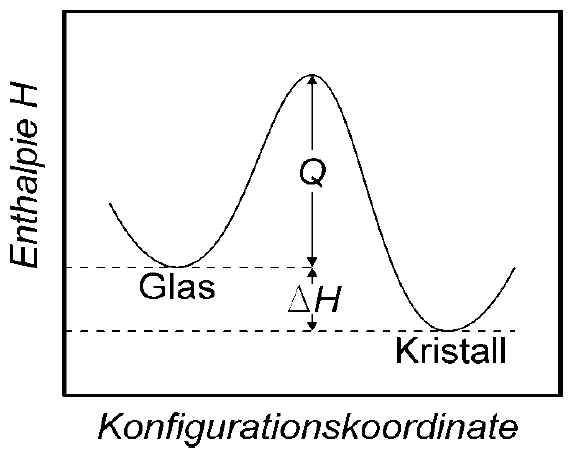
\includegraphics[width=0.7\linewidth]{img/kissinger}
		\caption{
			Kristallisationsenthalpie (H) und Aktivierungsenthalpie der Kristallisation (Q) eines amorphen Metalls. \cite{anleitung}
		}
		\label{fig_kissinger}
	\end{figure}

	\subsection{Röntgendiffraktometrie}
	%\subsubsection{Unsicherheiten} %hab ich bissle im Beob diskutiert.
	\subsubsection{Beobachtung und Datenanalyse}
	Die gemessenen Kurven sind in \cref{fig_xrd_kristallin} und \cref{fig_xrd_glas} dargestellt.
	Bei $\theta \approx \SI{31}{\degree}$ ist in der Messung der kristallinen Probe eine deutliche Kante zuerkennen.
	Sie kennzeichnet den Punkt an dem die Probe aus der Halterung gefallen ist und somit keine sinnvolle Messung mehr möglich war.
	Aus dem Abschnitt ohne Probe lässt sich die Unsicherheit durch den Untergrund abschätzen, da man ohne eine Probe keine Ereignisse erwartet.
	Jedoch ist die Schwankung während der Messung deutlich größer als die so abgeschätzte Unsicherheit, weshalb diese vernachlässigt werden kann.
	\begin{figure}[H]
			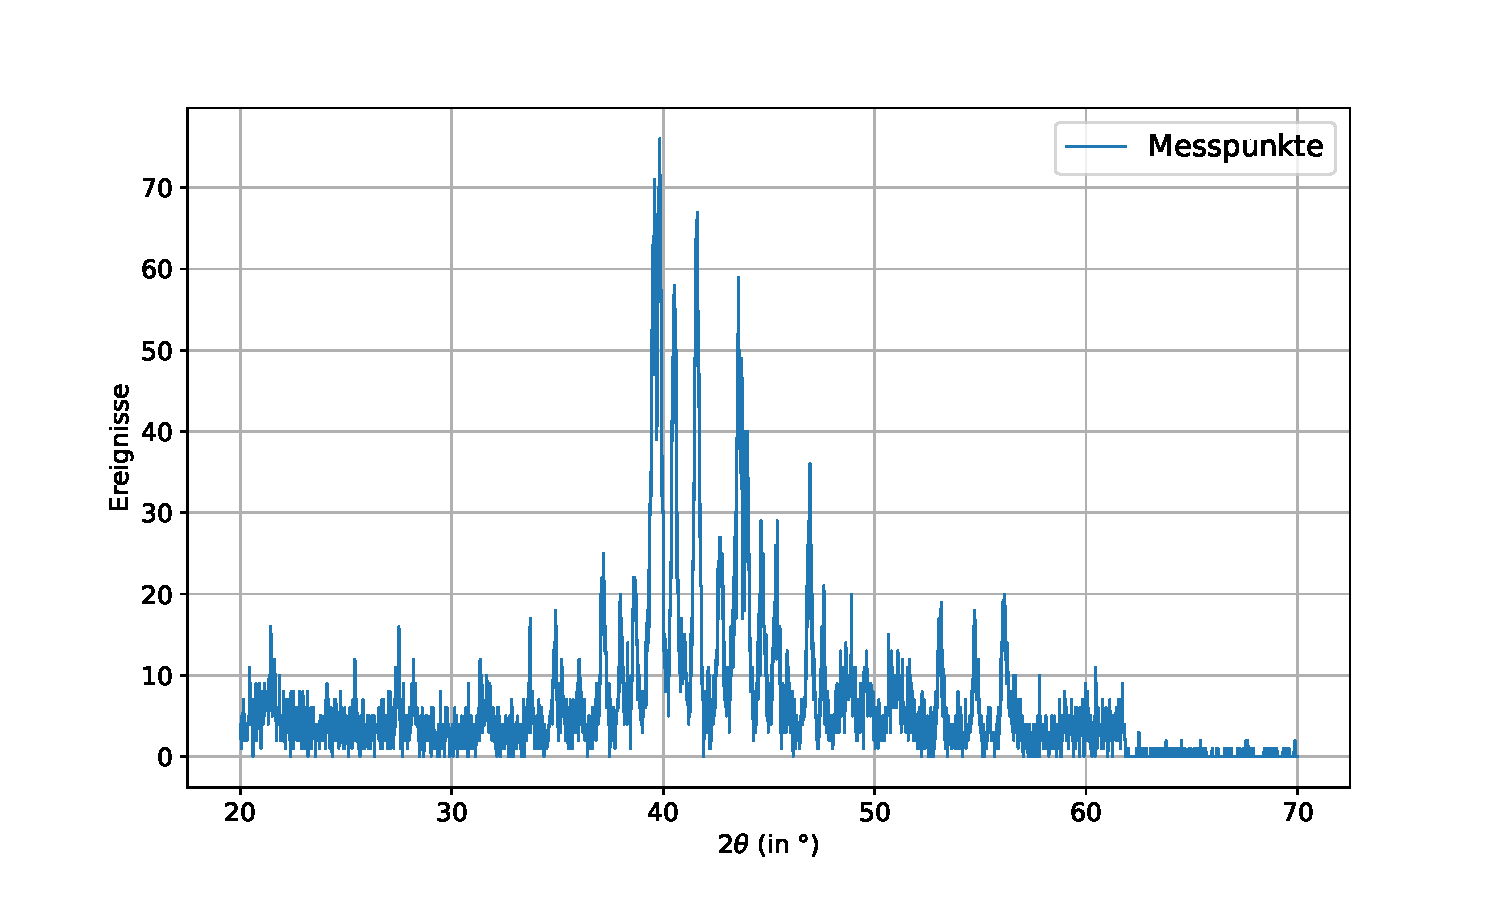
\includegraphics[width=\linewidth]{img/XRD_Kristallin_45_25.pdf}
			\caption{Diffraktogramm der kristallinen Probe.}
			\label{fig_xrd_kristallin}
	\end{figure}
	\begin{figure}[H]
			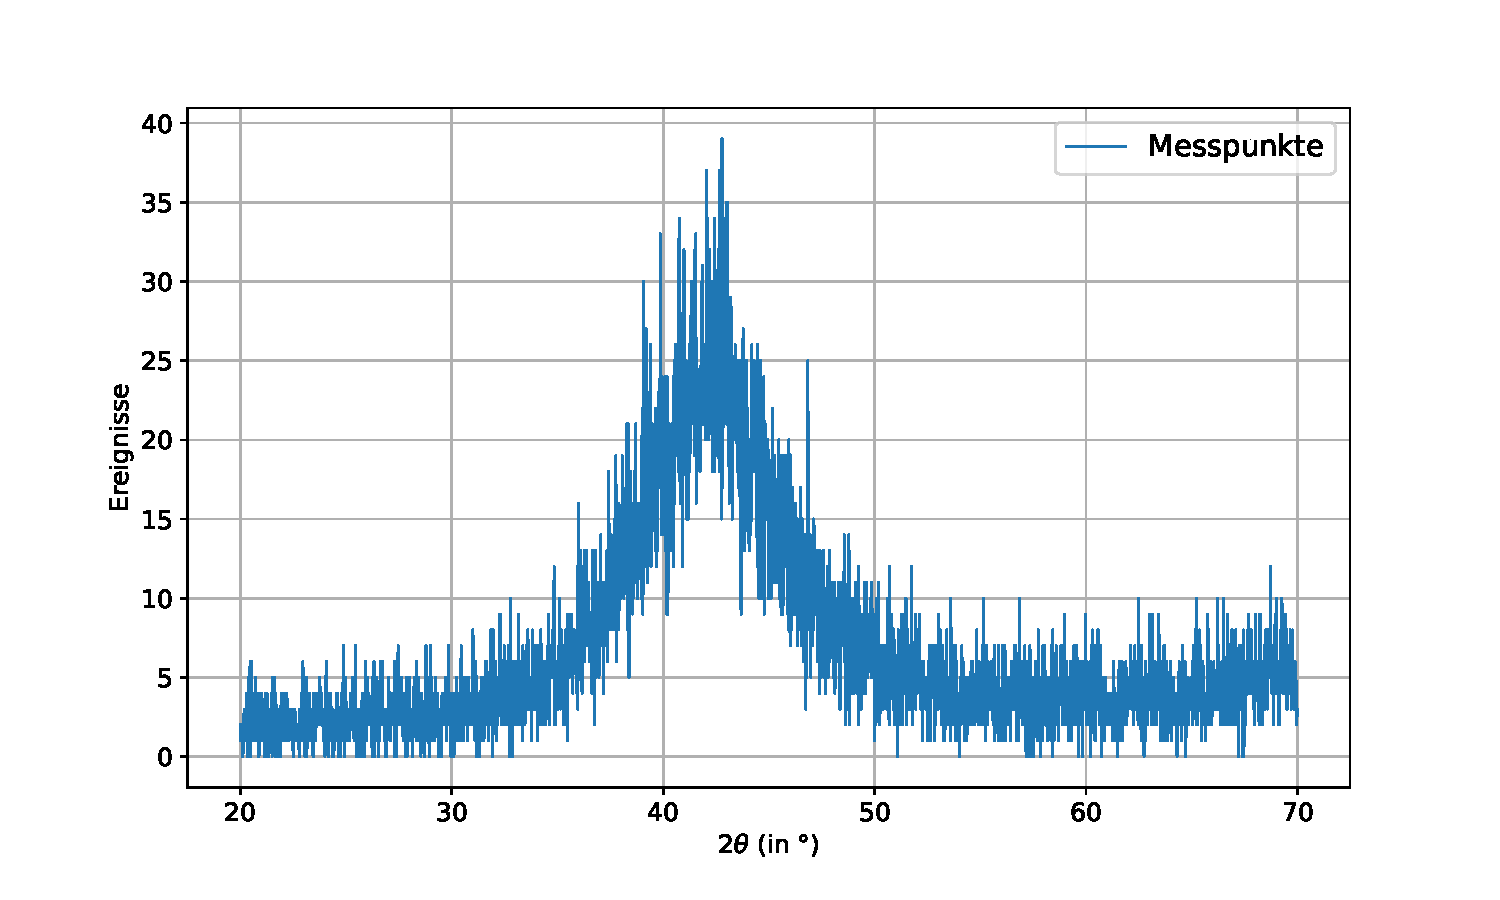
\includegraphics[width=\linewidth]{img/XRD_Glas_45_25.pdf}
			\caption{Diffraktogramm der Glasprobe.}
			\label{fig_xrd_glas}
	\end{figure}

	Zur Bestimmung der Positionen und Breiten der Peaks werden Gauß-Funktionen an die Messungen in einem Intervall um den Peak gefittet (vgl. \nameref{s_anhang}):
	\begin{equation}
		\label{eq_gauss}
		f(x) = a\cdot e^{-\frac{(x - c)^2}{2d^2}} + y
	\end{equation}
	Die gemittelten Peakpositionen der Proben befinden sich in \cref{tb_xrd_result}.
	Außerdem wurde nach der Bragg-\cref{eq_bragg} der Abstand der Gitterebenen, bzw. der mittler Atomabstand, berechnet.
	\begin{equation}
			\label{eq_bragg}
			\bar{d} = \frac{\lambda}{2\sin{\bar{\theta}}} \quad \text{mit} \quad u(\bar{d}) = \left|\frac{\cos{\bar{\theta}}}{2\sin^2{\bar{\theta}}} \right| \lambda \cdot u(\bar{\theta})
	\end{equation}
	Die Wellenlänge der Röntgenstrahlung der Kupfer-Anode beträgt $\lambda_{\text{K}_\alpha}= \SI{1.5406}{\angstrom}$.
	\begin{table}[H]
		\centering
		\begin{tabular}{ c | c | c | c | c | c}
			 Probe& Glas  &\multicolumn{4}{c}{Kristall} \\ \hline
			 Peak&  1 & 1 & 2 &  3 & 4\\ \hline
			 $2\bar{\theta}$ in \si{\degree}&\SI{42.2+-1.3}{}&\SI{39.7+-0.3}{} & \SI{40.52+-0.19}{} &\SI{41.59+-0.16}{} & \SI{43.6+-0.43}{} \\
			 $\bar{d}$ in \si{\angstrom} &\SI{2.14+-0.06}{} & \SI{2.27+-0.02}{} & \SI{2.224+-0.010}{} & \SI{2.17+-0.008}{} & \SI{2.07+-0.02}{}
		\end{tabular}
		\caption{Positionen der Diffraktogramm Peaks, sowie die aus der Bragg-\cref{eq_bragg} resultierenden Gitterebenenabstände (Kristall), bzw. der mittlere Atomabstand (Glas).}
		\label{tb_xrd_result}
\end{table}
	\subsubsection{Diskussion}
	% Anleitung sagt 3 maximalsten peaks, würde ich dann halt die schöneren 3 der 4 nehmen, oder alle weil ca. gleich hoch
	Rein qualitativ lässt sich sofort feststellen, dass erwartungsgemäß das Spektrum vom metallischen Glas in \cref{fig_xrd_glas} kontinuierlich ist, während das des Kristalls in \cref{fig_xrd_kristallin} eher diskret ist, was zeigt, dass die Glasprobe tatsächlich amorph ist.
	\cite{SIETSMA1991146} gibt die Atomabstände in \cref{tb_xrd_vgl} aus einer Kombination aus theoretischer Berechnung mit radialen Verteilungsfunktionen und experimenteller Bestimmung.
	Sie lassen sich nicht eindeutig den Messwerten in \cref{tb_xrd_result} zuordnen, da in der durchgeführten Messung nicht zwischen Atomsorten unterschieden werden kann. Der Messwert liegt aber zwischen den Literaturwerten für die einzelnen Atome, weshalb hier kein Widerspruch gezeigt werden kann. %TODO komisch vormuliert, ab idk
%TODO "kristallinen Proben ist mit Literaturdaten der Atomradien von Pd, Ni und P zu vergleichen (gewichteter Mittelwert)." << Anleitung, gewichteter Mittelwert? womit gewichtet, Masse,Voumen?

	\begin{table}[H]
		\centering
		\begin{tabular}{ c | c | c | c }
			 Peak&  $\sigma_1$ & $\sigma_2$ & $\sigma_3$\\ \hline
			  Atomdurchmesser & Pd \SI{2.8}{\angstrom} & Ni \SI{2.4}{\angstrom} & P \SI{1.8}{\angstrom}
		\end{tabular}
		\caption{Die in \cite{SIETSMA1991146} für Glas (PdNiP) angegebenen Atomdurchmesser. Sie wurden dort als beste Übereinstimmung von Experiment und Berechnung gewählt. Da mit Atomdurchmesser hier der Platz gemeint ist, den das Atom im Gitter einnimmt, ist er hier als mittlerer Atomabstand zu verstehen. Die Unsicherheit beträgt etwa \SI{0.005}{\angstrom}.} % das ist bissl riskant, weil ich nicht 100% sicher bin, ob das true ist.
		\label{tb_xrd_vgl}
\end{table}

	%TODO ich finde keinen Literaturwert für PdNiP in kristallförmig.
	%Die Größe der Schwankungen könnte dadurch zustande kommen, dass
	%TODO Absorption? naja. Drehprozess? Ist der ruckartig? misst der dazwischen?
	%TODO warum sind die Schwankungen so riesig?

	\subsection{Messung der Vickershärte}
	\subsubsection{Unsicherheiten} \label{sss_vicker_unsicher}
	Die Vickershärte wird direkt am Mikroskop von einer Digitalanzeige abgelesen.
	Mit einer Rechteckverteilung ergibt sich eine Unsicherheit von $u(H) = \SI{0.03}{HV}$.
	\subsubsection{Beobachtung und Datenanalyse}
	%TODO mehr Text hier
	In \cref{fig_indents} sind beispielhafte Aufnahmen des Mikroskops der zwei untersuchten Proben dargestellt.
	\begin{figure}[H]
		\centering
			\subcaptionbox{
				PdNiP-Probe.\label{fig_indent_pdnip}}{
			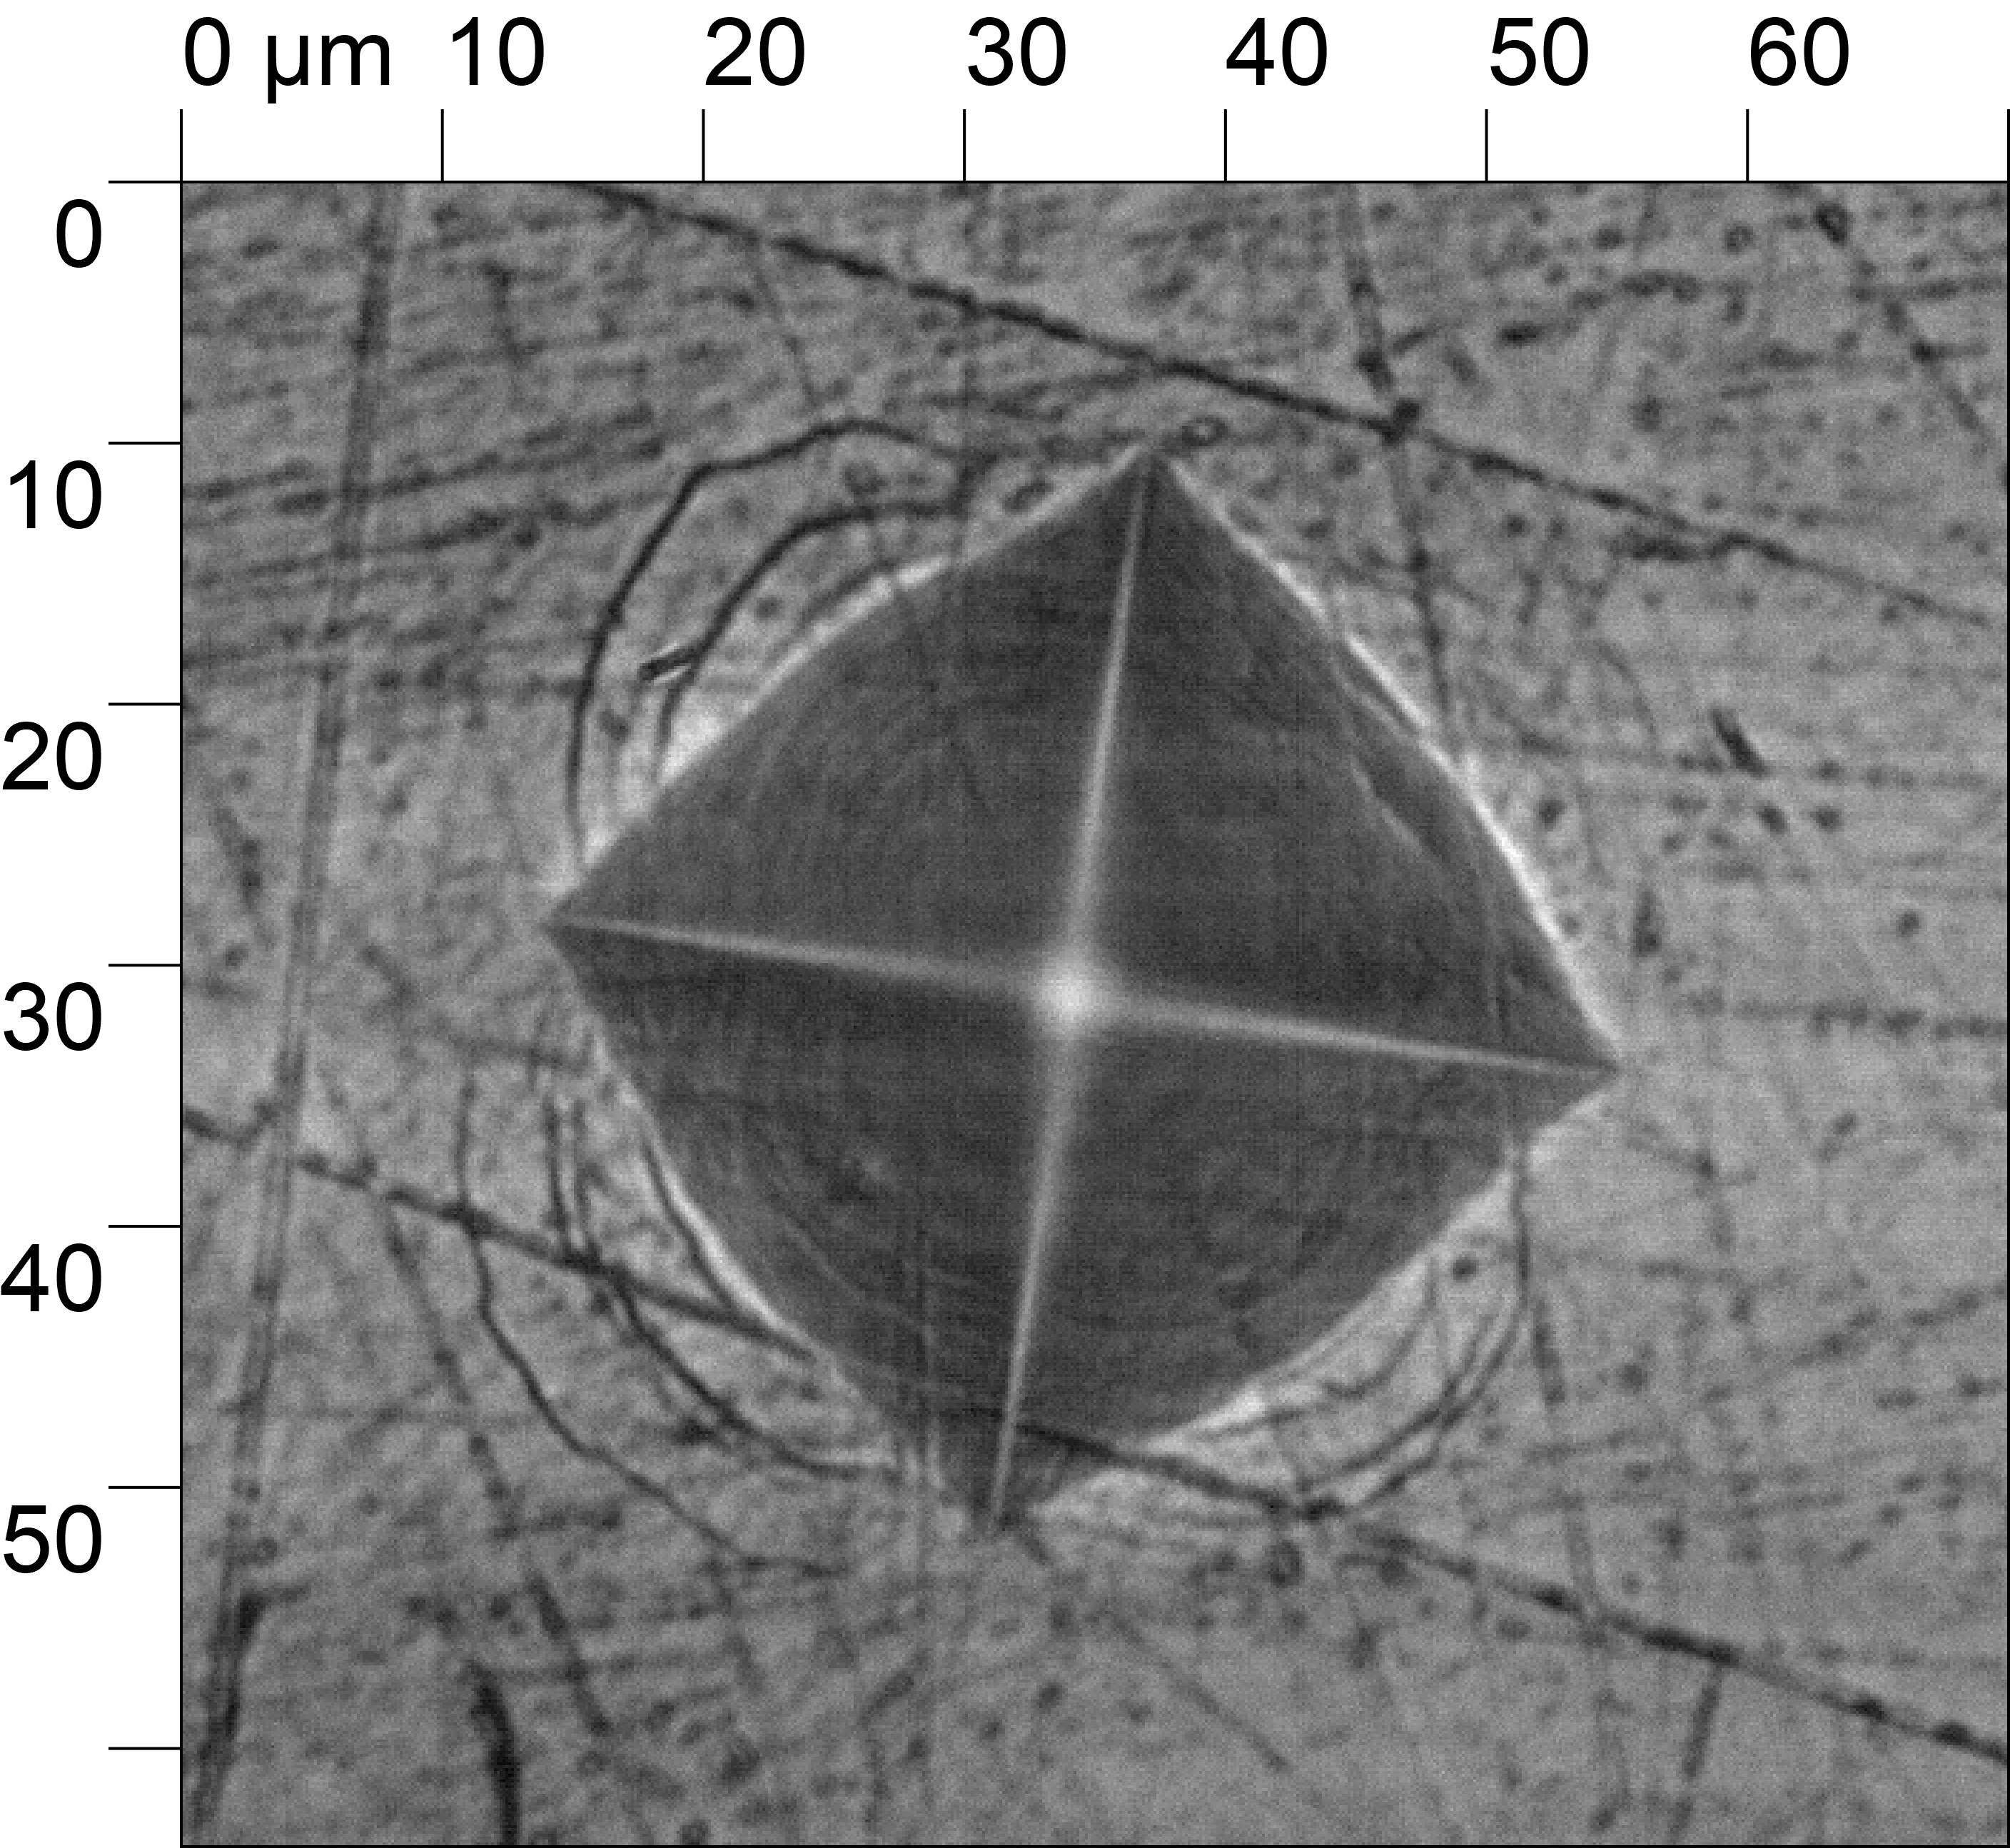
\includegraphics[width=.47\linewidth]{img/Paradin-Phosphor-500N-5s-l}}
			\subcaptionbox{
				Nickel-Probe.\label{fig_indent_ni}}{
			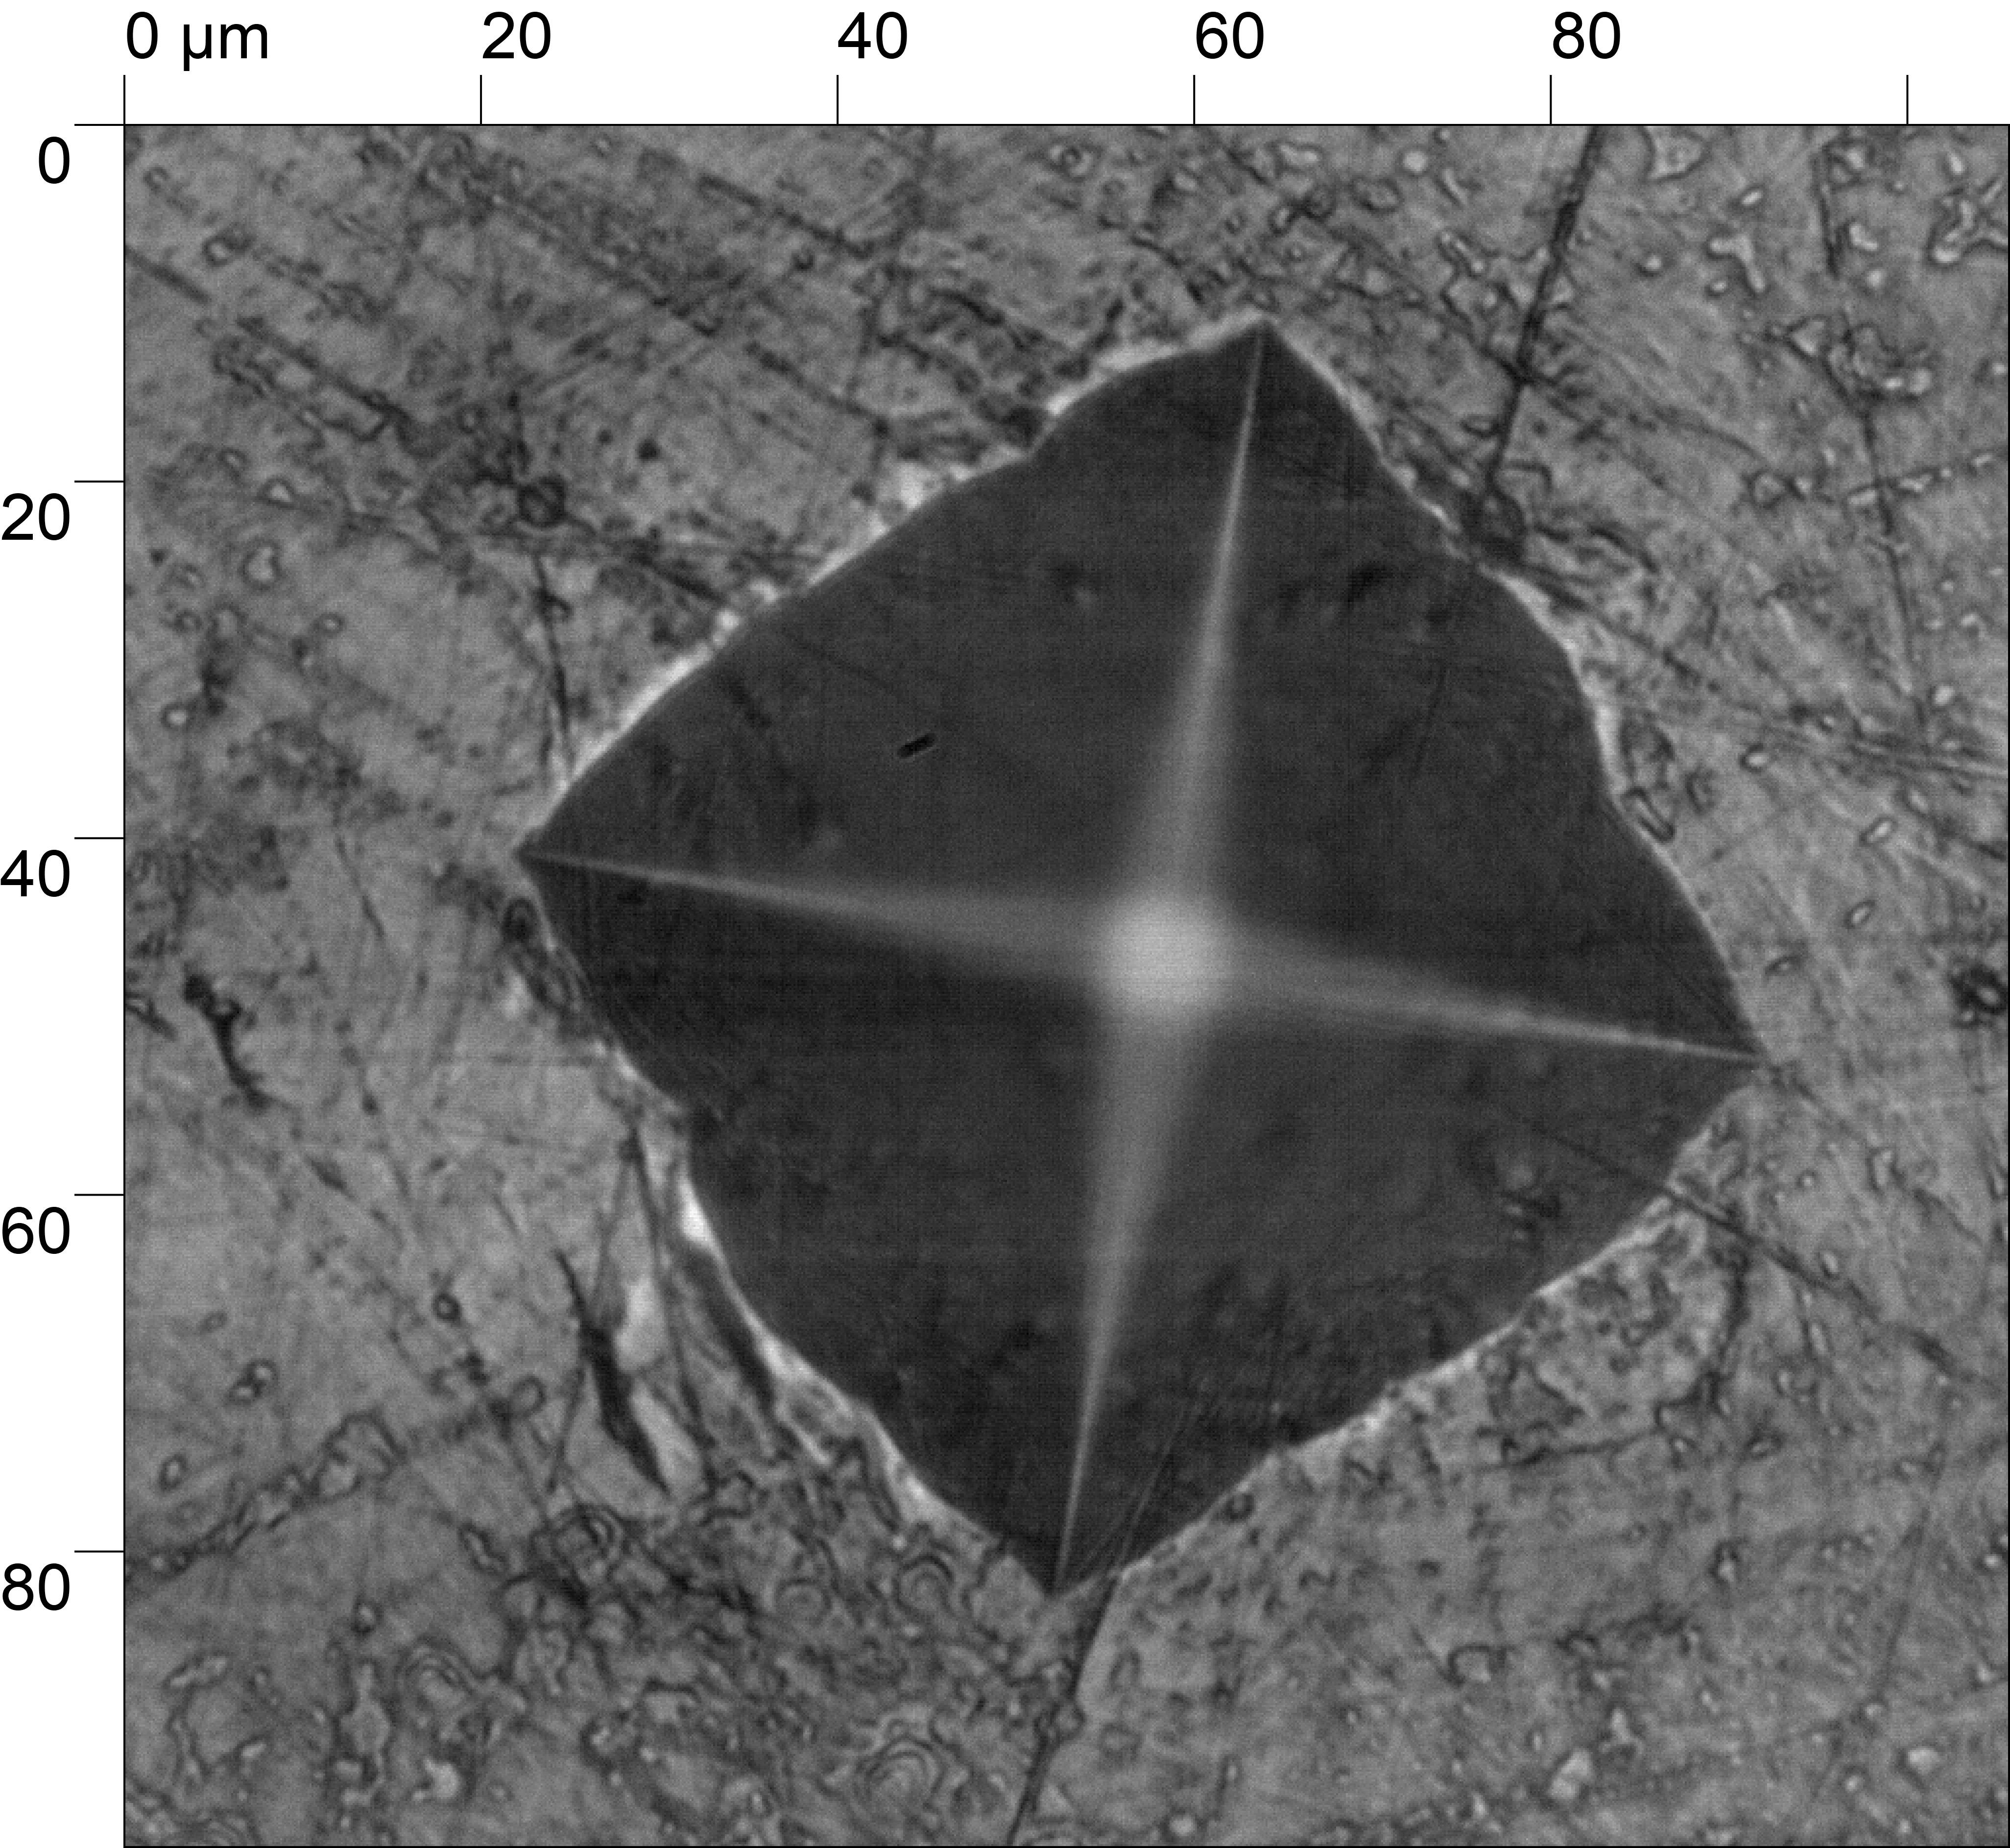
\includegraphics[width=.47\linewidth]{img/Ni-500N-5s-l}}
			\caption{Abdrücke der Indenterpyramide auf verschiedenen Proben. Der Fokus ist auf die Probenebene gelegt, weshalb die Mitte des Abdrucks unscharf ist.}
			\label{fig_indents}
 \end{figure}
 Der Mittelwert $\bar{H}$ von N Messungen berechnet sich nach GUM wie folgt:
 \begin{equation}
	 \bar{H} = \frac{1}{N}\sum_{i=1}^N H_i \quad \text{mit} \quad u(\bar{H}) = \sqrt{\sum_{i=1}^N \frac{(H_i-\bar{H})^2}{N-1}}
 \end{equation}
 Die gemittelte Vickershärte der Nickel-Probe beträgt \SI{188+-5}{HV} und die der PdNiP-Probe \SI{534+-14}{HV}.
 Die Unsicherheit durch die Digitalanzeige (vgl. \ref{sss_vicker_unsicher}) verschwindet gegenüber der Standardabweichung der Mittelwerte.

	\subsubsection{Diskussion}
	% Bilder vergleichen, dass erwähnen was er meinte mit man sieht schön die 'Brechung'/'Verschiebung' oder so, kp was es war
	% wie erwartet Glas härter

	In \cref{fig_indents} ist zu erkennen, dass bei der PdNiP-Probe dauerhafte Verformungen außerhalb des Pyramidenabdrucks auftreten.
	In der Nickel-Probe ist das nicht der Fall.
	Dies liegt daran, dass im Kristall bei einer Verformung die geschobenen Atome einfach einige Gitterpositionen weiter springen können, ohne die Gitterstruktur zu verletzen. %TODO 'springen'
	Im amorphen PdNiP ist dies nicht möglich, weshalb Bereiche unterschiedlicher Nahordnung ebenfalls geschoben werden und die beobachteten \enquote{ripples} auftreten. %TODO ripple fine? >> IMO Ja, aber 'anderer Nahordnung' klingt komisch
	Diese leichtere Verschiebbarkeit der Atome im Kristall im Vergleich zum amorphem Glas ist auch der Grund dafür, dass die PdNiP-Probe die beobachtete deutlich höhere Vickershärte (\SI{524 \pm 14}{HV}) als die kristalline Nickel-Probe (\SI{188 \pm 5}{HV}) hat.

	%TODO Notes für Diskussion v , weil abgetrennt >>???

	\section{Schlussfolgerung}
	% Rückgriff auf Hypothese und drittes Nennen dieser
	Die Versuche zum Vergleich von gläserner und kristalliner Phase von Metallen konnten viele der Erwartungen bestätigen.
	Die Untersuchung des Wärmeflusses mit einem Leistungskalorimeter hat die Bestimmung der Schmelz- und Erstarrungsenthalpie von Blei erlaubt und es konnte gezeigt werden, dass dieser Vorgang reversibel ist.
	Ebenfalls bestimmt werden konnte die Kristallisationsenthalpie von PdNiP und bestätigt werden, dass die Kristallisation des gläsernen PdNiPs irreversibel ist.
	Die Bestimmung der Aktivierungsenthalpie nach Kissinger wäre exakter möglich, indem Thermogramme für weitere Heizraten gemessen werden würden.

	Die Möglichkeit der Zuordnung von zwei PdNiP-Proben zur kristallinen und gläsernen Phase durch Pulverdiffraktometrie konnte auch gezeigt werden.
	Die Bestimmung der Gitter- bzw. mittleren Atomabstände war möglich, aber konnte nicht eindeutig bestätigt werden.

	Die Vickershärte der amorphen PdNiP- und kristallinen Nickelprobe wurde bestimmt und es wurde gezeigt, dass die Glasphase eine größere Härte aufweist.

	% Quellen zitieren, Websiten mit Zugriffsdatum
	% Verweise auf das Laborbuch (sind erlaubt)
	% Tabelle + Bilder mit Beschriftung
	\printbibliography
	\section{Anhang} \label{s_anhang}
	%TODO image sizes/scaling 2 Bilder auf 1 Seite?
	\subsection{Röntgendiffraktometrie}

	\begin{figure}[H]
			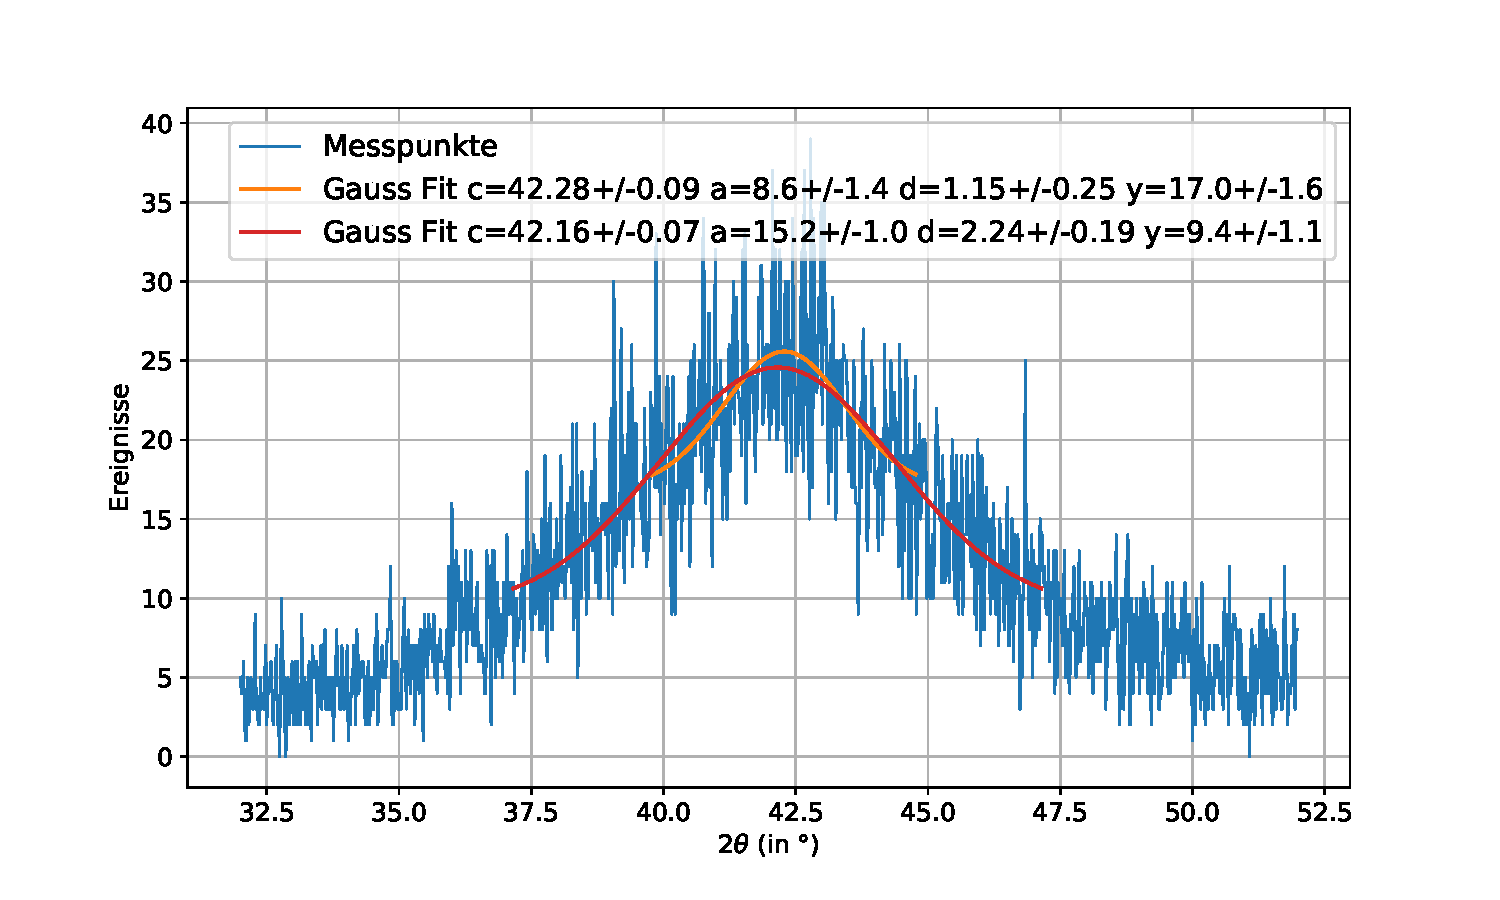
\includegraphics[width=\linewidth]{img/XRD_Glas_42_10.pdf}
			\caption{
				Vergrößertes Diffraktogramm der Glasprobe.
				Die Fitfunktionen sind Gauß-Funktionen nach \cref{eq_gauss}.
				Die für den Fit einbezogenen Messpunkte entstammen dem Intervall, in welchem die jeweilige Gauß-Funktion abgebildet ist.
				}
			\label{fig_xrd_glas_1}
	\end{figure}



	\begin{figure}[H]
			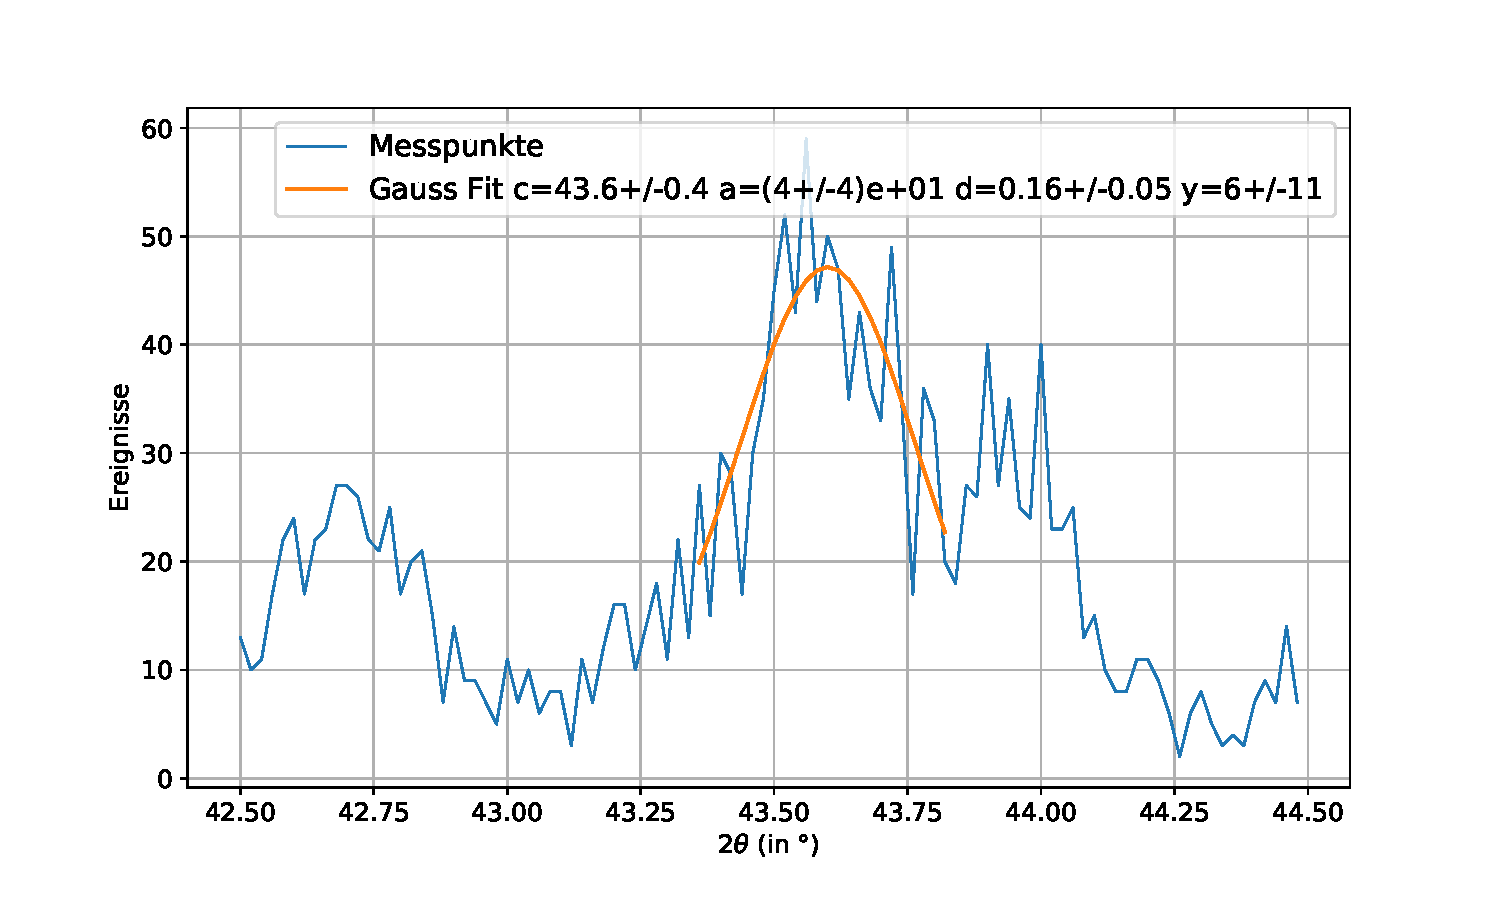
\includegraphics[width=\linewidth]{img/XRD_Kristallin_43,5_1.pdf}
			\caption{
				Vergrößertes Diffraktogramm der kristallinen Probe.
				Die Fitfunktionen sind Gauß-Funktionen nach \cref{eq_gauss}.
				Die für den Fit einbezogenen Messpunkte entstammen dem Intervall, in welchem die jeweilige Gauß-Funktion abgebildet ist.
				}
			\label{fig_xrd_kristall_1}
	\end{figure}
	\begin{figure}[H]
			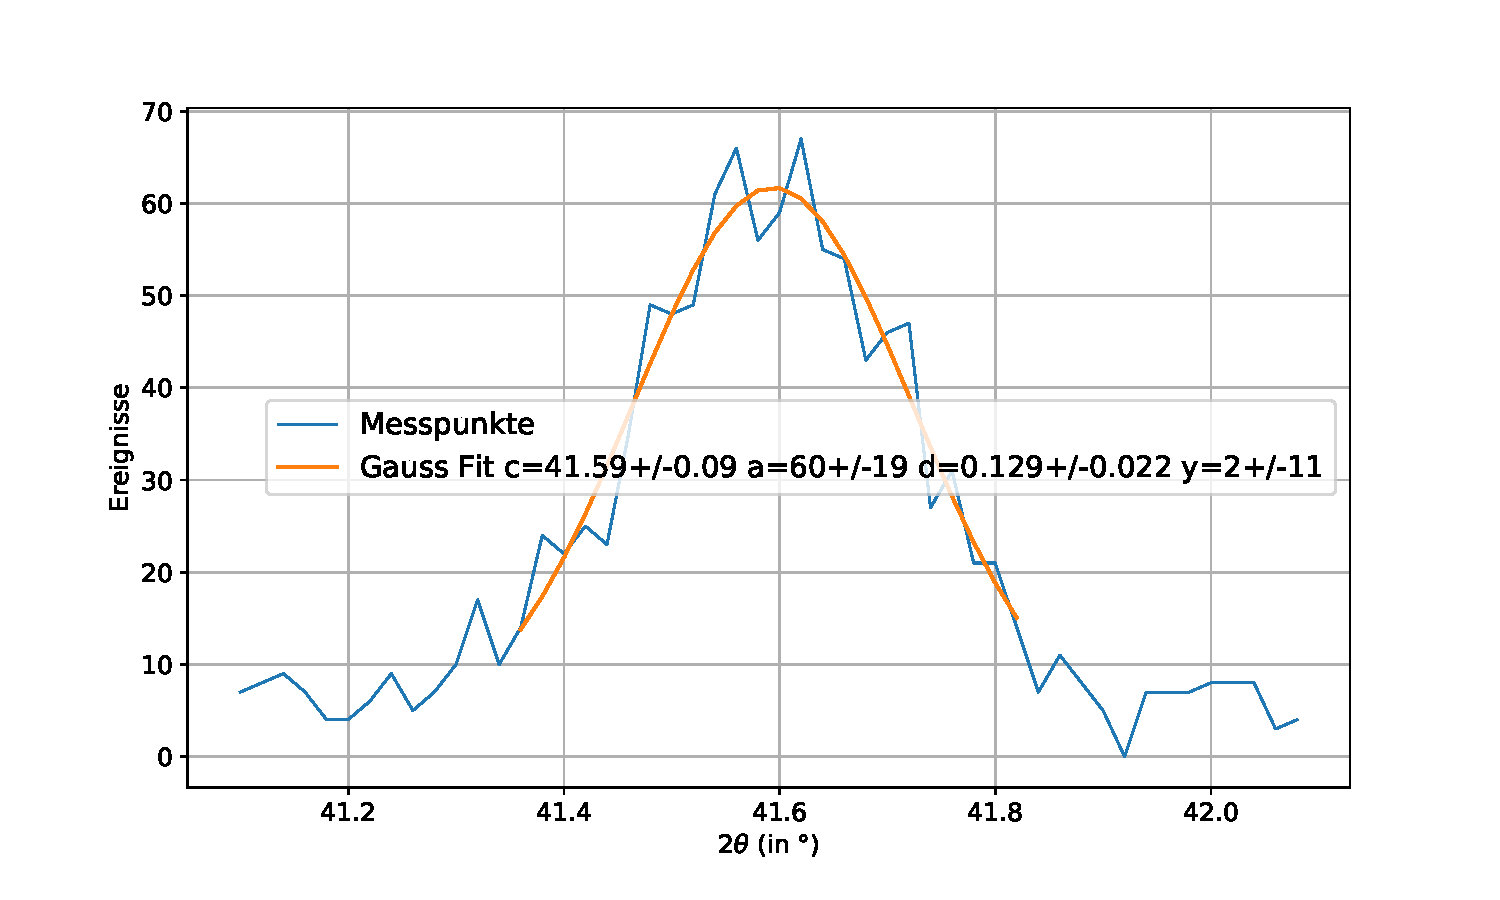
\includegraphics[width=\linewidth]{img/XRD_Kristallin_41,6_0,5.pdf}
			\caption{
				Vergrößertes Diffraktogramm der kristallinen Probe.
				Die Fitfunktionen sind Gauß-Funktionen nach \cref{eq_gauss}.
				Die für den Fit einbezogenen Messpunkte entstammen dem Intervall, in welchem die jeweilige Gauß-Funktion abgebildet ist.
				}
			\label{fig_xrd_kristall_2}
	\end{figure}
	\begin{figure}[H]
			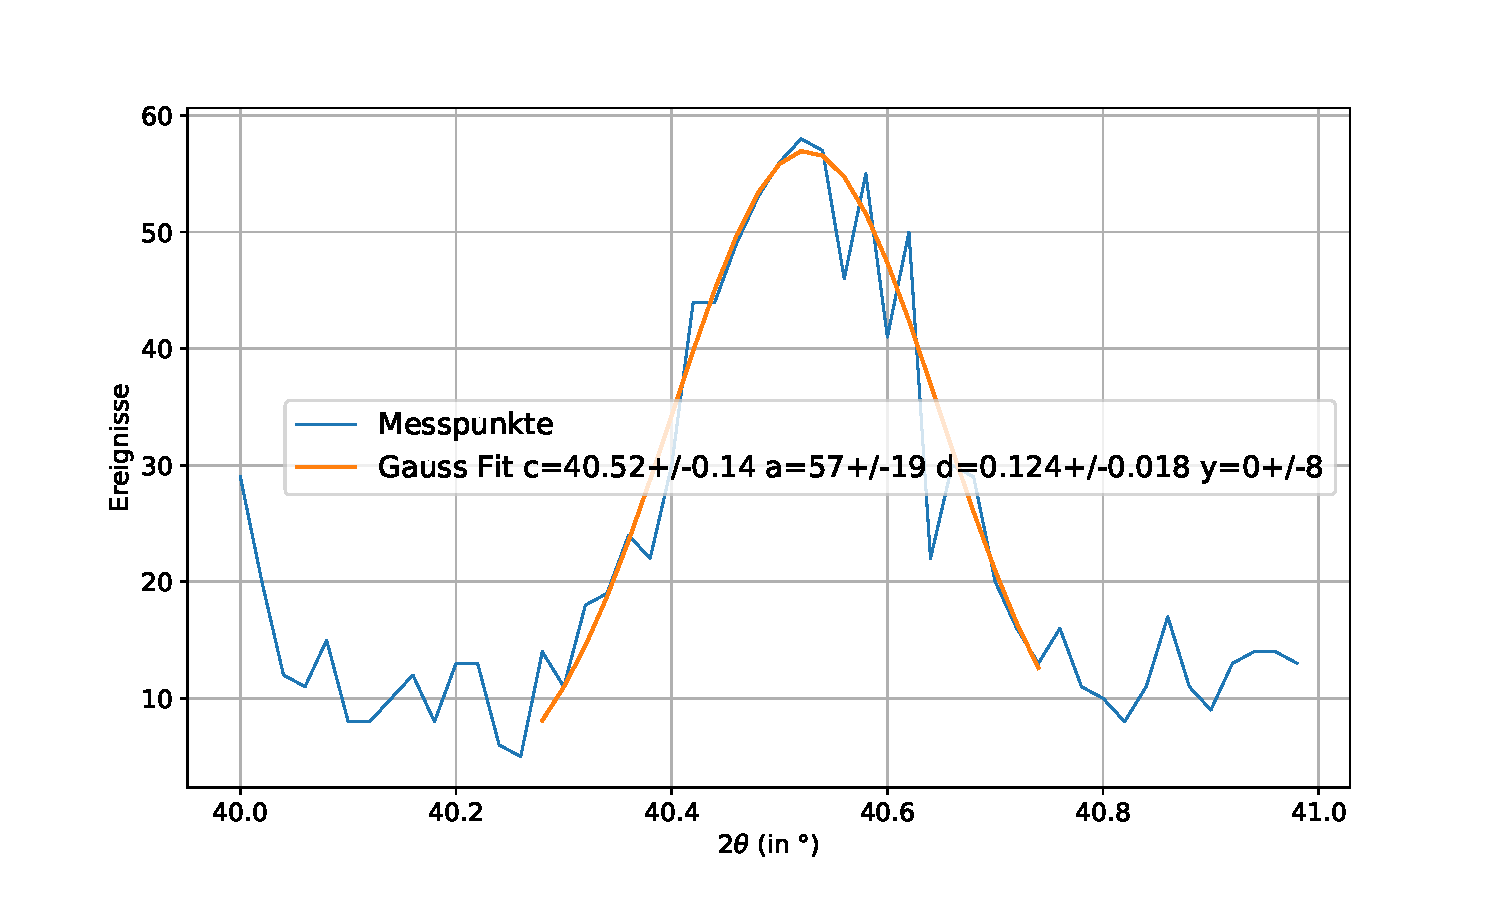
\includegraphics[width=\linewidth]{img/XRD_Kristallin_40,5_0,5.pdf}
			\caption{
				Vergrößertes Diffraktogramm der kristallinen Probe.
				Die Fitfunktionen sind Gauß-Funktionen nach \cref{eq_gauss}.
				Die für den Fit einbezogenen Messpunkte entstammen dem Intervall, in welchem die jeweilige Gauß-Funktion abgebildet ist.
				}
			\label{fig_xrd_kristall_3}
	\end{figure}
	\begin{figure}[H]
			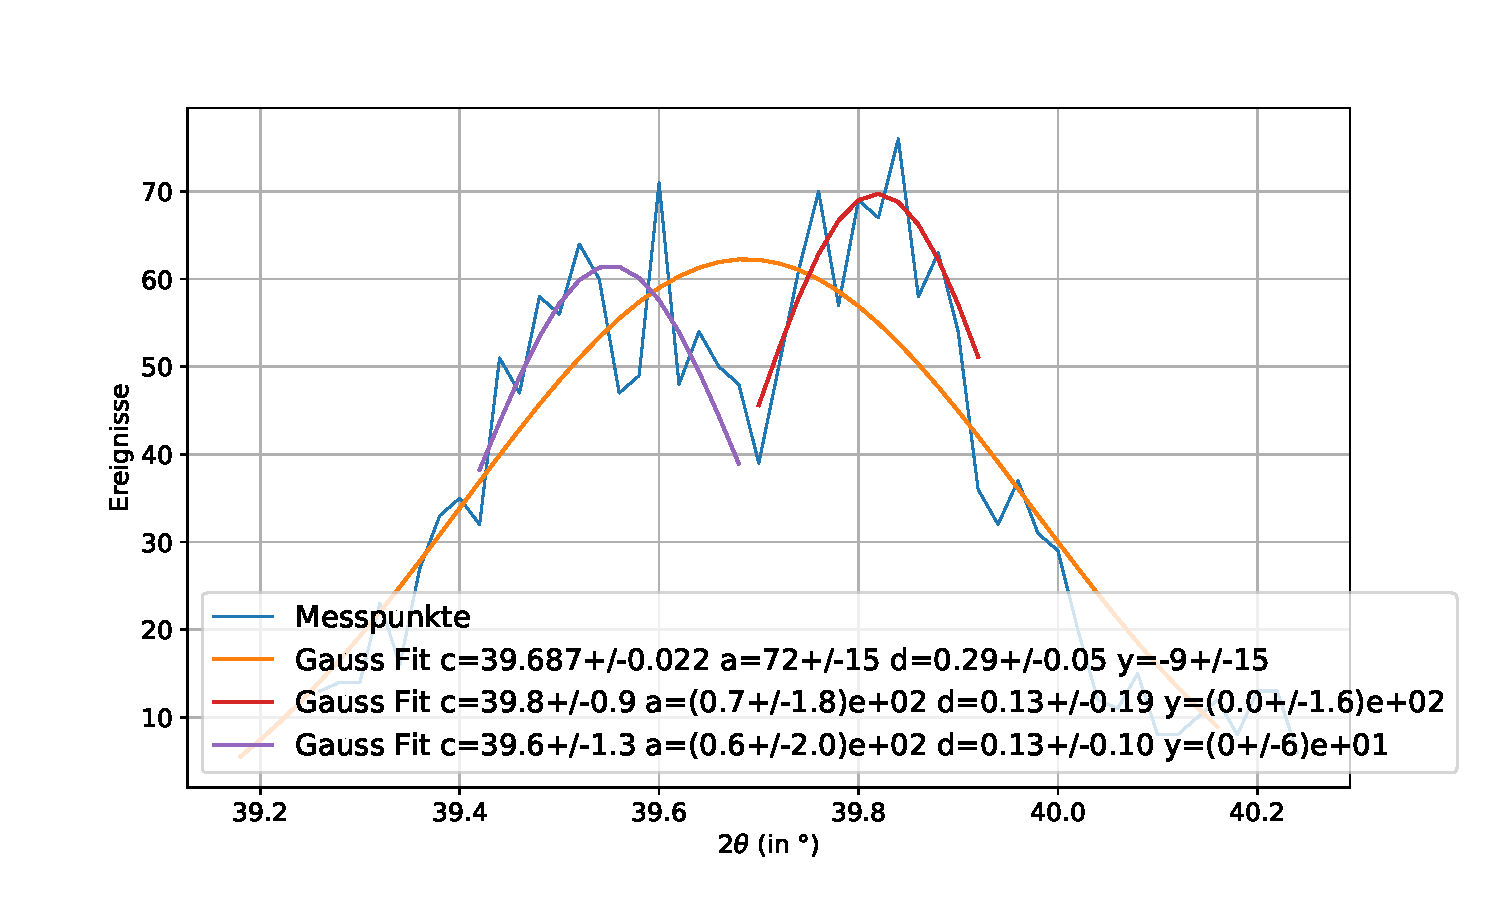
\includegraphics[width=\linewidth]{img/XRD_Kristallin_39,76_0,5.pdf}
			\caption{
				Vergrößertes Diffraktogramm der kristallinen Probe.
				Die Fitfunktionen sind Gauß-Funktionen nach \cref{eq_gauss}.
				Die für den Fit einbezogenen Messpunkte entstammen dem Intervall in welchem die jeweilige Gauß-Funktion abgebildet ist.
				}
			\label{fig_xrd_kristall_4}
	\end{figure}
\end{document}
